\documentclass[a4paper]{article}

\author{Misrraim~Su\'arez~P\'erez}
\title{FirstMarket}



\usepackage[utf8]{inputenc}
\usepackage[spanish,es-tabla,es-nodecimaldot,es-lcroman]{babel}

\usepackage{csquotes}
\linespread{1.25}

\usepackage{graphicx}
\graphicspath{ {./images/} }

\usepackage{xcolor}

\usepackage{listings}
\lstdefinelanguage{JavaScript}{
	keywords={typeof, new, true, false, catch, function, return, null, catch, switch, var, if, in, while, do, else, case, break, let, const},
	keywordstyle=\color{blue}\bfseries,
	ndkeywords={class, export, boolean, throw, implements, import, this},
	ndkeywordstyle=\color{darkgray}\bfseries,
	identifierstyle=\color{black},
	sensitive=false,
	comment=[l]{//},
	morecomment=[s]{/*}{*/},
	commentstyle=\color{purple}\ttfamily,
	stringstyle=\color{olive}\ttfamily,
	morestring=[b]',
	morestring=[b]"
}
\lstset{
	language=JavaScript,
	backgroundcolor=\color{lightgray},
	extendedchars=true,
	basicstyle=\footnotesize\ttfamily,
	showstringspaces=false,
	showspaces=false,
	numbers=left,
	numberstyle=\footnotesize,
	numbersep=9pt,
	tabsize=2,
	breaklines=true,
	showtabs=false,
	captionpos=b
}


\usepackage{hyperref}
\hypersetup{
	colorlinks=true,
	linkcolor=blue,
	filecolor=magenta,      
	urlcolor=cyan,
}

\urlstyle{same}



\begin{document}

    \maketitle
    \tableofcontents

    % INTRODUCCION
    \section{Introducción}
    El presente proyecto se enmarca dentro del Proyecto Final de Grado correspondiente al Grado en Ingeniería Informática de la Universidad Nacional de Educación a Distancia.
    
    Se basa en el proyecto específico ofertado por el Departamento de Sistemas de Comunicación y Control de la UNED titulado \emph{Desarrollo de un portal de comercio electrónico}. Citando la propia descripción de dicha oferta de proyecto específico:
    
    \begin{displayquote}
        El proyecto consiste en el desarrollo de un portal web orientado al comercio electrónico. Dicha aplicación permitirá al comprador seleccionar artículos, realizar pedidos y pagos a través de una pasarela. El sistema también ofrecerá al comerciante gestionar los artículos expuestos en el portal.
    \end{displayquote}

	En este contexto, el comercio electrónico desarrollado a sido una librería, denominada \textbf{FirstMarket}.

    \subsection{Motivación y Objetivos}
    Desde un primer momento la intención fue desarrollar un proyecto que tuviese la mayor relación posible con el mercado actual, lo que, junto con un fuerte interés personal hacia el ecosistema de Internet, llevó a la decisión de escoger esta propuesta.
    
    La idea era desarrollar algo moderno, útil, con reflejo real en la sociedad y que cumpliese el papel de facilitar la inserción laboral. En este sentido, las aplicaciones web en general, y las específicas de comercio electrónico en particular, cumplen a la perfección los requisitos comentados. A nadie se le escapa hoy en día la implantación casi ubicua que estas tecnologías tienen en la sociedad.
    
    Por otro lado, y en clara conexión con lo comentado, otro objetivo de este último trabajo del plan de estudios fue el de servir como \emph{compensador} final de lagunas formativas. En este sentido, el control de versiones con Git era una tarea pendiente inaplazable, así como profundizar en tecnologías web básicas como HTTP, HTML, CSS ó JavaScript. Además, ampliar el dominio de las tecnologías Java siempre fue algo muy deseable.
    
    Conviene no dejar de lado, por obvio, que un objetivo fundamental del presente trabajo es el de dar fin al plan de estudios. Remarcar esto es relevante porque en múltiples situaciones puede entrar en conflicto con la intención de desarrollar una aplicación web lo más moderna posible. Como se explicará más adelante en esta memoria, el mundo de las tecnologías web es muy cambiante, y pretender desarrollar una aplicación web alineada con el estado del arte en la materia partiendo, como es el caso, desde prácticamente cero conocimientos, sale fuera del marco de un trabajo de estas características. Por tanto, siempre se ha tenido en cuenta un compromiso entre recursos disponibles (principalmente tiempo y conocimientos) y grado de modernidad en las tecnologías usadas.
    \\
    
    En definitiva, el principio fundamental que ha guiado la toma de decisión ha sido el reforzar, y alinear en la medida de lo posible con el estado del arte, las habilidades técnicas adquiridas fruto del plan de estudios, de forma a facilitar una futura integración en la industria web, a la par de satisfacer una histórica inquietud personal en la materia.


    \subsection{Internet, Web y Aplicaciones Web}
    En esta sección se ofrece una introducción, meramente descriptiva, del contexto en el que situar la aplicación web desarrollada. Se tratará de diferenciar los conceptos de Internet, World Wide Web y aplicaciones web.

    \subsubsection{¿Qué es Internet?}
    Tal como se explica en [bib ref], esta pregunta puede ser enfocada desde dos puntos de vista complementarios.
    
    Por un lado, desde una perspectiva \textbf{hardware}, Internet es una red que conecta miles de millones de dispositivos en todo el mundo, denominados \emph{hosts} o \emph{sistemas finales}, por medio de \emph{enlaces de comunicación} y \emph{conmutadores de paquetes}.
    
    Los enlaces de comunicación son diferentes tipos de medios físicos a través de los cuales se transfieren ondas electromagnéticas que portan la información. Puede tratarse de medios guiados, como cables de cobre, cables coaxiales o fibra óptica, o no guiados, como el espectro de radio. Cuando un sistema final decide enviar información a otro sistema final, el emisor fragmenta los datos en \emph{paquetes} de información y los envía al destinatario a través de la red. Una vez en destino, el sistema final receptor ensambla los paquetes para reconstruir los datos originales. Un conmutador de paquetes toma un paquete que llega a uno de sus enlaces de comunicación entrantes y decide hacia cuál de sus enlaces de comunicación salientes lo reenvía.
    
    Estas \emph{redes de conmutación de paquetes} se pueden entender de forma análoga a una empresa que necesita mover una gran cantidad de carga entre dos almacenes separados gran distancia. En el almacén de origen la carga se divide y organiza en diferentes contenedores. Cada uno de los contenedores viaja de forma independiente a través de la red de transporte disponible siguiendo posiblemente rutas no del todo iguales. Por ejemplo, unos contenedores pueden ir por ciertas carreteras en ciertos camiones mientras que otros pueden viajar en tren o incluso en barco, o cualquier combinación de los anteriores. Lo importante es la independencia entre la ruta de un contenedor concreto con los demás. Una vez llegados al almacén de destino, la carga se extrae de los contenedores y se agrupa con el resto que llega del mismo envío. Así, los paquetes son análogos a los contenedores, los enlaces de comunicación son análogos a las vías de transporte, los conmutadores de paquetes son análogos a las intersecciones o discontinuidades en las vías de transporte (piénsese en una simple rotonda), y los sistemas finales son análogos a los almacenes. Pues bien, de igual forma que un contenedor toma un camino a través de la red de transporte, un paquete de información toma un camino a través de la infraestructura de Internet.
    
    Por otro lado, es posible describir Internet desde un punto de vista \textbf{software} como un servicio prestado a las aplicaciones distribuidas, es decir, como una interfaz de programación que las aplicaciones distribuidas consumen.
    
    Se dice que las aplicaciones son aplicaciones distribuidas, o \textbf{aplicaciones de Internet}, cuando se ejecutan en diferentes máquinas que intercambian datos entre sí. Es importante destacar que las aplicaciones de Internet se ejecutan estrictamente en los sistemas finales, no en la infraestructura de la red, que es agnóstica (o debiera serlo) de la semántica de la información que está trasportando. Así, puede pensarse en Internet como un servicio postal, que garantiza el envío de información entre partes, las cuales pueden estar desarrollando cualquier tipo de actividad basada, entre otras cosas, en la propia comunicación que mantienen. Al igual que el servicio postal impone una serie de reglas para ser usado, como dónde depositar la carta que se pretende enviar o dónde y de qué manera especificar la dirección de envío, Internet ofrece unas reglas en forma de interfaz de programación que las aplicaciones de Internet deben adoptar.
    
    \subsubsection{¿Qué es la Web?}
    Siguiendo el hilo de la discusión del epígrafe anterior, la World Wide Web es una de las muchas aplicaciones de Internet existentes. Otras serían el correo electrónico, las aplicaciones para acceder remotamente a otra máquina, la transferencia de archivos, el streaming de video, la telefonía por Internet, y más.
    
    A veces, dado que la Web es la aplicación más conocida, se confunde la parte con el todo al identificarla con la propia Internet. Sin embargo, esta aplicación surgió bastante tiempo después de que otras ya estuvieran ampliamente implantadas y maduras, como el correo electrónico o la transferencia de ficheros, si bien su uso era principalmente en ámbitos académicos.
    
    Lo que da tanta importancia a la Web es que fue la aplicación de Internet que, a principios de los años 90, abrió al gran público a la hasta entonces desconocida Internet. De hecho, esta aplicación llevó a Internet de ser tan sólo una más de muchas redes existentes a ser la dominante por excelencia.
   
   	Entonces, como se ha dicho, la Web es una aplicación de Internet, y como tal se trata de software que se ejecuta en diferentes máquinas que intercambian mensajes entre sí. El formato de estos mensajes, su timing y demás \emph{reglas de conversación} se recogen en un protocolo, el HyperText Transfer Protocol (HTTP). Este protocolo es el corazón de la Web, encontrándose definido en [RFC 1945] y en [RFC 2616], y su implementación se materializa en dos programas ejecutados en diferentes sistemas finales, un programa cliente y un programa servidor.
    
    La mecánica básica gira en torno a peticiones y respuestas. El programa cliente envía un mensaje HTTP conteniendo una petición al programa servidor. Por su parte, siguiendo las reglas definidas en el protocolo, el programa servidor contesta enviando otro mensaje HTTP al cliente. En el caso más común, el cliente le solicita al servidor el envío de una \emph{página web}.
    
    Una página web es un documento de texto escrito con unas reglas de sintaxis específicas. Estas reglas definen el Hypertext Markup Language (HTML). En el sistema final cliente, la página web es presentada en pantalla de una manera amigable al usuario por medio de programas que procesan el contenido en HTML.
    
    En definitiva, y sin entrar en matices que desvíen de la esencia, la Web es la aplicación de Internet que permite el consumo de páginas web bajo demanda por parte de los usuarios (en contraste con el modelo broadcast, en el que se emite y el usuario sólo puede consumir lo emitido, como en la radio).
    
    \subsubsection{¿Qué es una Aplicación Web?}
    
    %A web application is defined as a hierarchy of directories and files in a standard layout. Such a hierarchy can be accessed in its "unpacked" form, where each directory and file exists in the filesystem separately, or in a "packed" form known as a Web ARchive, or WAR file. The former format is more useful during development, while the latter is used when you distribute your application to be installed.
    
    
    %The complete syntax and semantics for the deployment descriptor is defined in Chapter 13 of the Servlet API Specification, version 2.3.
    
    Las páginas web que son enviadas desde el servidor al cliente se dice que pueden ser estáticas o dinámicas. Esta característica, más que hablar de la página web en sí misma, habla del proceso mediante el cual su contenido ha sido creado y modificado a lo largo del tiempo.
   	
   	Las páginas estáticas lo son en el sentido de que su contenido, creado comúnmente por un humano, no varía con el tiempo de manera programática. La información que presentan es la misma, a menos que se modifique \emph{a mano}. Así eran todas las páginas web en los primeros años. En contraste, en las páginas web dinámicas, el contenido no está dado de antemano, sino que se genera en cada ciclo de petición-respuesta. Esto es útil porque entre otras cosas permite páginas web personalizadas para cada usuario, e incluso que sea él mismo quien aporte contenido a la página web.
    
    Una \textbf{aplicación web} es el sistema software encargado de la generación dinámica de páginas webs. Normalmente, y a diferencia del modelo estático, entre sus componentes se encuentra una base de datos que permita la persistencia de la información, cambiante por definición de la propia arquitectura.
    
    Desde este punto de vista, en el presente proyecto se ha desarrollado una aplicación web encargada de generar contenido web que los usuarios pueden visitar con el objetivo de comprar libros a través de Internet.

    \subsection{Estructura de la Memoria}
    Estructura

    % ANALISIS
    \section{Análisis}

        \subsection{Requisitos}

            La aplicación debe admitir los roles y capacidades siguientes:
            \begin{enumerate}
                \item Usuario anónimo (UA).
                \begin{itemize}
                    \item[-] Por defecto, al acceder al sitio web se hace como UA, sin ninguna validación ni credencial. Basta con acceder a la URL de inicio de la aplicación.
                    \item[-] Un UA debe poder realizar búsquedas de libros, es decir, debe tener pleno acceso a la exploración del catálogo.
                    \item[-] La plena exploración del catálogo debe permitir realizar búsque\-das filtradas según 0, 1 o más criterios, tales como: categoría, título o autor.
                    \item[-] Un UA debe poder visualizar información detallada de un libro, por ejemplo de entre los obtenidos tras una búsqueda.
                    \item[-] Un UA debe poder consultar las promociones disponibles.
                    \item[-] Un UA debe poder registrarse en el sistema completando un formulario (nombre, contraseña, dirección de correo electrónico, etc.).
                    \item[-] Finalizado el proceso de registro, el nuevo UR debe recibir confirmación por correo electrónico.
                    \item[-] En su caso, un UA debe poder iniciar sesión en el sistema.
                    \item[-] En su caso, un UA debe poder realizar el procedimiento de recuperación de contraseña.
                \end{itemize}
                \item Usuario registrado (UR). Este perfil representa a un usuario que ha pasado de anónimo a registrado. Un UR posee todas las capacidades del UA, más otras específicas suyas, a saber:
                \begin{itemize}
                    \item[-] Poder editar la información de su perfil de usuario.
                    \item[-] Realizar pedidos y efectuar los correspondientes pagos a través de una pasarela segura.
                    \item[-] Disponer de una cesta virtual para la gestión de la compra.
                    \item[-] En la cesta se debe poder introducir, modificar la cantidad o eliminar libros (esto último de uno en uno o todos a la vez).
                    \item[-] En cualquier momento del proceso de realizar un pedido, el UR debe poder cancelarlo.
                    \item[-] Tras una compra, el UR debe recibir confirmación en su correo electrónico.
                    \item[-] Un UR debe poder consultar el estado de sus pedidos.
                    \item[-] Puntuar (de alguna manera, p.e. estrellas del 1 al 5) un determinado libro que haya adquirido. Debe poder hacerlo en cualquier momento tras la compra.
                    \item[-] Consultar un histórico de sus transacciones, detallando los libros comprados, la fecha de la compra y el precio de cada uno.
                    \item[-] Darse de baja como UR.
                    \item[-] Cerrar sesión.
                    \item[-] Un UR debe poder ponerse en contacto con el administrador de la aplicación web a través de un formulario de contacto, recibiendo confirmación por correo electrónico tras el envío del mismo.
                \end{itemize}
                \item Usuario Administrador
                \begin{itemize}
                    \item[-] Ver y editar (añadir, modificar, eliminar) la jerarquía de categorías (CRUD categorías).
                    \item[-] Ver y editar (añadir, modificar, eliminar) la información relativa a los libros (título, autor/es, editorial, precio, disponibilidad, \ldots) (CRUD libros).
                    \item[-] Crear, modificar o eliminar promociones de libros (CRUD promociones).
                    \item[-] Tener acceso a la información de los UR, salvo sus contraseñas.
                    \item[-] Bloquear-desbloquear a un UR.
                    \item[-] Visualizar la información de los pedidos, tanto los que estén en curso como los finalizados.
                    \item[-] Poder alterar el estado de un pedido.
                    \item[-] Poder generar informes (p.e. ventas durante un determinado periodo con su importe y la facturación total).
                \end{itemize}
            \end{enumerate}

            Además de lo anterior, la aplicación debe:
            \begin{enumerate}
                \item[a)] Garantizar la persistencia de los datos referentes a UR, pedidos, pagos, productos y sus categorías.
                \item[b)] Mostrar un mensaje de error cuando un usuario introduzca incorrectamente sus credenciales de autenticación.
            \end{enumerate}

        \subsection{Casos de Uso}
            En este apartado se presentan las interacciones más comunes que los usuarios pueden realizar con la aplicación web. No se pretende proporcionar una enumeración exhaustiva de todos los casos de uso, sino un subconjunto relevante de los mismos, a modo de introducción a las capacidades básicas que se espera de la aplicación.

            \begin{figure}[htb!]
                \centering
                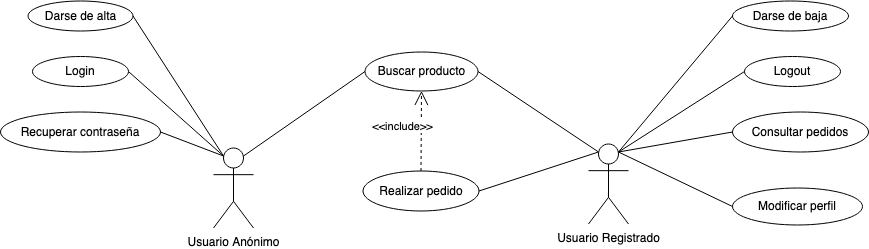
\includegraphics[width=\textwidth]{use-case_diagram}
                \caption{Diagrama de casos de uso}
                \label{fig:use-case_diagram}
            \end{figure}

            \subsubsection{CU01\_Búsqueda}
            Proceso por el cual un usuario explora el catálogo y acaba por visualizar la página de un libro.
            \begin{itemize}
                \item[+] Actores implicados: Usuario Anónimo, Usuario Registrado.
                \item[+] Precondiciones: Usuario situado en cualquiera de las páginas que dan acceso al catálogo.
                \item[+] Flujo principal:
                \begin{enumerate}
                    \item[1.] El usuario hace click en alguna de las categorías principales mostradas a modo de catálogo flotante en la barra de navegación
                    o hace click en \emph{All Books}.
                    \item[2.] El sistema muestra la página de resultados de búsqueda.
                    \item[3.] El usuario hace click en alguno de los productos mostrados.
                    \item[4.] El sistema muestra la página del libro.
                \end{enumerate}
                \item[+] Flujo alternativo: \emph{refinamiento\_búsqueda}. El usuario altera en la página de resultados algún criterio de filtro.
                \begin{itemize}
                    \item[3.b.] El usuario selecciona/deselecciona algún criterio de filtro de entre los mostrados en la página de resultados de búsqueda.
                    \item[4.b.] El sistema vuelve al punto 2 del flujo principal.
                \end{itemize}
                \item[+] Flujo alternativo: \emph{búsqueda\_por\_texto}. El usuario introduce una cadena de texto en el cuadro de búsqueda.
                \begin{itemize}
                    \item[1.b.] El usuario introduce una cadena de texto en el cuadro de búsqueda y hace click en buscar.
                \end{itemize}
            \end{itemize}

            \subsubsection{CU02\_Alta}
            Proceso por el cual se crea un nuevo usuario registrado.
            \begin{itemize}
                \item[+] Actores implicados: Usuario Anónimo.
                \item[+] Flujo principal:
                \begin{enumerate}
                    \item[1.] El usuario hace click en el link de nuevo registro, disponible en la página de \emph{login}.
                    \item[2.] El sistema presenta un formulario donde introducir la dirección de email y la contraseña.
                    \item[3.] El usuario introduce y envía la información pedida.
                    \item[4.] El sistema comprueba la información proporcionada.
                    \item[5.] El sistema crea una nueva cuenta de usuario, pero la mantiene inactiva a la espera de confirmar la dirección de email.
                    \item[6.] El sistema envía un email con un link de confirmación a la dirección proporcionada, e informa al usuario por pantalla.
                    \item[7.] El usuario accede a su email y hace click en el link enviado, confirmando que la dirección de email es suya.
                    \item[8.] El sistema activa la cuenta de usuario.
                    \item[9.] El sistema envía al usuario un email de bienvenida.
                    \item[10.] El sistema redirige al usuario a la página de \emph{login}.
                \end{enumerate}
                \item[+] Flujo alternativo: \emph{usuario\_ya\_registrado}. La dirección proporcionada se encuentra registrada en el sistema.
                \begin{itemize}
                    \item[5.b.] El sistema no crea una nueva cuenta de usuario. Por razones de seguridad, la manera en que el sistema informa al usuario tras esta situación es indistinguible del flujo principal, de forma que no se pueda deducir que ese email ya tiene cuenta asociada en el sistema.
                \end{itemize}
                \item[+] Flujo alternativo: \emph{link\_ya\_enviado}. El sistema está a la espera de la confirmación de un link válido en esta dirección de email.
                \begin{itemize}
                    \item[5.b.] El sistema no crea una nueva cuenta de usuario. Se informa al usuario acerca de una condición de error \-{}genérica, por seguridad\- en relación con la dirección de email proporcionada, pidiéndose que compruebe su dirección de email.
                \end{itemize}
                \item[+] Flujo excepcional: \emph{time\_out}. El usuario no confirma su dirección de email dentro de un plazo determinado.
                \begin{itemize}
                    \item[7.b.] El sistema detecta el timeout e invalida el link de confirmación enviado. Si el usuario hace click en el link caducado se le informa de dicha condición.
                \end{itemize}
            \end{itemize}

            \subsubsection{CU03\_Login}
                Proceso por el cual un usuario se autentica en el sistema.
                \begin{itemize}
                    \item[+] Actores implicados: Usuario Anónimo.
                    \item[+] Flujo principal:
                    \begin{enumerate}
                        \item[1.] El usuario hace click en el link de \emph{login}, o intenta realizar alguna operación que requiera autenticación (por ejemplo, añadir un libro a la cesta).
                        \item[2.] El sistema presenta el formulario de acceso (dirección de email y la contraseña).
                        \item[3.] El usuario introduce y envía la información pedida.
                        \item[4.] El sistema comprueba las credenciales.
                        \item[5.] El sistema redirige al usuario a la página principal.
                    \end{enumerate}
                    \item[+] Flujo alternativo: \emph{fallo\_autenticación}. El email no se encuentra registrado en el sistema, o la contraseña proporcionada no es correcta.
                    \begin{itemize}
                        \item[5.b.] El sistema informa al usuario acerca de un fallo genérico de autenticación, de forma que, por razones de seguridad, no se pueda deducir si el email proporcionado se encuentra registrado en el sistema.
                    \end{itemize}
                    \item[+] Flujo alternativo: \emph{bloqueo\_cuenta}. El usuario anónimo realiza, dentro de un marco de tiempo (configurable), un número de intentos (configurable) de login con contraseña errónea.
                    \begin{itemize}
                        \item[5.b.] El sistema bloquea la cuenta asociada al email para prevenir ataques por fuerza bruta.
                        \item[6.] El sistema informa al usuario por pantalla y mediante el envío de un email.
                        \item[7.] Pasado el tiempo de seguridad (configurable), el sistema desbloquea la cuenta del usuario.
                    \end{itemize}
                    \item[+] Post-Condiciones: El usuario pasa a tener rol de usuario registrado en el sistema.
                \end{itemize}

            \subsubsection{CU04\_RecuperarContraseña}
                Un usuario previamente registrado en el sistema intenta acceder al mismo, pero no recuerda su contraseña. El sistema intentará crear una nueva contraseña y enviarla al e-mail del usuario.
                \begin{itemize}
                    \item[+] Actores implicados: Usuario Anónimo.
                    \item[+] Flujo principal:
                    \begin{enumerate}
                        \item El usuario hace click en la opción \emph{¿olvidó su contraseña?}.
                        \item El sistema presenta un formulario donde introducir la dirección de email.
                        \item El usuario introduce y envía su dirección de email.
                        \item El sistema comprueba la dirección de email.
                        \item Comprobación correcta. El sistema envía un email con un link de confirmación a la dirección proporcionada, e informa de ello al usuario por pantalla.
                        \item Link no caducado. El usuario accede a su email y hace click en el link, confirmando que efectivamente la dirección proporcionada es la suya.
                        \item El sistema genera una nueva contraseña y se la asigna al usuario.
                        \item El sistema envía la nueva contraseña a la dirección de email del usuario, y le avisa de ello por pantalla.
                    \end{enumerate}
                    \item[+] Flujo alternativo: \emph{usuario\_no\_registrado}. La dirección proporcionada no se encuentra registrada en el sistema.
                    \begin{itemize}
                        \item[5.b.] El sistema no envía correo alguno pero, por razones de seguridad, desde el punto de vista del usuario este flujo alternativo es indistinguible del principal.
                    \end{itemize}
                    \item[+] Flujo excepcional: \emph{time\_out}. El usuario no confirma su dirección de email dentro de un plazo determinado.
                    \begin{itemize}
                        \item[6.b.] El sistema detecta el timeout e invalida el link de confirmación enviado. Si el usuario hace click en el link caducado se le informara de dicha condición.
                    \end{itemize}
                \end{itemize}

            \subsubsection{CU05\_EditarPerfil}
                Proceso por el cual un usuario modifica alguno de los datos de su perfil personal.
                \begin{itemize}
                    \item[+] Actores implicados: Usuario Registrado.
                    \item[+] Flujo principal:
                    \begin{enumerate}
                        \item[1.] El usuario hace click en \emph{área personal}.
                        \item[2.] El sistema muestra la página de área personal, en donde se muestra el formulario de datos personales, rellenado con la información actual del usuario.
                        \item[3.] El usuario modifica los datos del formulario y lo envía al sistema.
                        \item[4.] El sistema comprueba los datos.
                        \item[5.] Comprobación correcta.El sistema actualiza la información del usuario.
                        \item[6.] El sistema muestra la página de inicio.
                    \end{enumerate}
                    \item[+] Flujo alternativo: \emph{error\_datos\_formulario}. Los datos proporcionados en el formulario de información personal no son válidos.
                    \begin{itemize}
                        \item[5.b.] El sistema regresa al punto 3 del flujo principal, e informa al usuario acerca del fallo producido.
                    \end{itemize}
                    \item[+] Flujo alternativo: \emph{cancelar}. El usuario cancela el proceso de edición de su información personal.
                    \begin{itemize}
                        \item[3.b.] El usuario hace click en el botón \emph{cancelar}. El sistema muestra la página de inicio.
                    \end{itemize}
                    \item[+] Post-Condiciones: El usuario ha alterado su información personal almacenada en la aplicación.
                \end{itemize}

            \subsubsection{CU06\_RealizarPedido}
                Proceso por el cual un usuario realiza una compra a través de la aplicación web.
                \begin{itemize}
                    \item[+] Actores implicados: Usuario Registrado.
                    \item[+] Precondiciones: Desde cualquier página en la que se muestren libros (página de inicio, página de resultados de búsqueda o página de un libro) el usuario hace click en \emph{add to cart}, para uno o mas libros.
                    \item[+] Flujo principal:
                    \begin{enumerate}
                        \item[1.] El usuario hace click en el icono de la cesta.
                        \item[2.] El sistema muestra la página de la cesta del usuario, con todos los libros contenidos en el mismo.
                        \item[3.] El usuario puede aumentar o disminuir el número de unidades de un libro, o incluso eliminarlo por completo, y hace click en \emph{checkout}.
                        \item[4.] El sistema comprueba la disponibilidad de los libros contenidos en la cesta.
                        \item[5.] Stock suficiente. El sistema muestra la página de checkout, con el formulario de datos de envío y pago, y el resumen de la compra.
                        \item[6.] El usuario completa los datos de envío y de pago y hace click en \emph{Pay}.
                        \item[7.] El sistema tramita el pago.
                        \item[8.] Pago ok. El sistema registra el nuevo pedido.
                        \item[9.] El sistema confirma al usuario por pantalla y por email que el pedido se ha realizado con éxito.
                    \end{enumerate}
                    \item[+] Flujo alternativo: \emph{stock\_insuficiente}. No hay stock suficiente para satisfacer el contenido de la cesta.
                    \begin{itemize}
                        \item[5.b.] El sistema vuelve al punto 2 del flujo principal, informando al usuario de los libros para los cuales no hay stock suficiente.
                        \item[3.b.] El usuario reduce la cantidad demandada de los libros correspondientes y hace click en \emph{checkout}.
                    \end{itemize}
                    \item[+] Flujo alternativo: \emph{error\_pago}. Error al efectuar el pago.
                    \begin{itemize}
                        \item[8.b.] El sistema vuelve al punto 5 del flujo principal, informando al usuario del problema respecto al pago.
                    \end{itemize}
                    \item[+] Flujo excepcional: \emph{libro\_eliminado}. Algún libro de la cesta ya no esta disponible en el sistema.
                    \begin{itemize}
                        \item[5.b.] El sistema elimina de la cesta automáticamente los libros que el administrador haya deshabilitado.
                        \item[6.b.] El sistema vuelve al punto 2 del flujo principal, informando al usuario de los libros que han sido eliminados.
                    \end{itemize}
                    \item[+] Post-Condiciones: El usuario ha efectuado un nuevo pedido.
                \end{itemize}

            \subsubsection{CU07\_ConsultarPedido}
                Proceso por el cual un usuario consulta el historial de pedidos que ha realizado.
                \begin{itemize}
                    \item[+] Actores implicados: Usuario Registrado.
                    \item[+] Flujo principal:
                    \begin{enumerate}
                        \item[1.] El usuario hace click en \emph{My Purchases} en la barra de navegación.
                        \item[2.] El sistema muestra la página de los pedidos del usuario.
                        \item[3.] El usuario puede expandir-contraer la información mostrada relativa a un pedido.
                    \end{enumerate}
                \end{itemize}

            \subsubsection{CU08\_Baja}
                Proceso por el cual un usuario elimina su cuenta de la tienda online.
                \begin{itemize}
                    \item[+] Actores implicados: Usuario Registrado.
                    \item[+] Flujo principal:
                    \begin{enumerate}
                        \item[1.] El usuario hace click en \emph{área personal}.
                        \item[2.] El sistema muestra la página de área personal.
                        \item[3.] El usuario selecciona \emph{eliminar cuenta}.
                        \item[4.] El sistema muestra el formulario de eliminación de cuenta.
                        \item[5.] El usuario completa y envía el formulario.
                        \item[6.] El sistema comprueba los datos.
                        \item[7.] Comprobación correcta. El sistema actualiza el estado del usuario y envía un email de confirmación.
                        \item[8.] El sistema muestra la página de inicio.
                    \end{enumerate}
                    \item[+] Flujo alternativo: \emph{error\_datos\_formulario}. La contraseña proporcionada en el formulario de baja no es correcta.
                    \begin{itemize}
                        \item[7.b.] El sistema regresa al punto 4 del flujo principal, e informa al usuario acerca del fallo producido.
                    \end{itemize}
                    \item[+] Flujo alternativo: \emph{cancelar}. El usuario cancela el proceso de baja.
                    \begin{itemize}
                        \item[5.b.] El usuario cancela el proceso de baja. El sistema regresa al punto 2 del flujo principal.
                    \end{itemize}
                    \item[+] Post-Condiciones: El usuario ya no figura como dado de alta en la aplicación.
                \end{itemize}

            \subsubsection{CU09\_Logout}
                Proceso por el cual un usuario cierra su sesión en el sistema.
                \begin{itemize}
                    \item[+] Actores implicados: Usuario Registrado.
                    \item[+] Precondiciones: el usuario está con su sesión abierta en el sistema.
                    \item[+] Flujo principal:
                    \begin{enumerate}
                        \item[1.] El usuario hace click en el link de \emph{logout}.
                        \item[2.] El sistema cierra la sesión del usuario.
                        \item[3.] El sistema muestra la página de inicio.
                    \end{enumerate}
                    \item[+] Post-Condiciones: El usuario ha efectuado el logout con éxito.
                \end{itemize}


    % DISEÑO
    \section{Diseño}
    En este apartado se ofrece una descripción de las decisiones tomadas a nivel de diseño de la aplicación web.
    \subsection{Arquitectura del Sistema}
    Desde un punto de vista lo suficientemente alejado como para no percibir los detalles internos, la aplicación web está organizada siguiendo la arquitectura clásica cliente-servidor-datos. Hoy en día, quizás, esta no sea la organización más vanguardista. Los términos \emph{serverless}, \emph{microservicios} o \emph{single-page-application} son los que con mayor eco resuenan en la industria web actual.
    
    \begin{figure}[h]
    	\centering
    	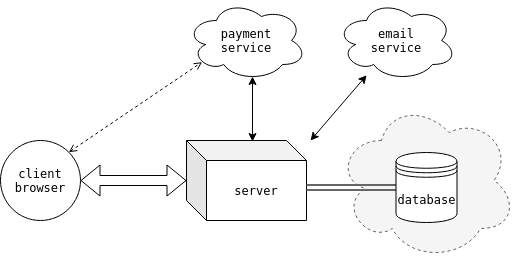
\includegraphics[width=\textwidth]{desing_general}
    	\caption{Modelo del sistema}
    	\label{fig:desing_general}
    \end{figure}
    
    Como muchas tendencias dentro del mundo de la computación, estos términos no están del todo delimitados, ofreciendo en ocasiones diferentes interpretaciones y/o solapamientos entre sí. Serverless hace mención a aquellas aplicaciones web que en su mayor parte, o por completo, incorporan servicios cloud de terceras partes para gestionar su propia lógica de negocio. La arquitectura de microservicios está muy relacionada con lo anterior, ya que esta concibe las aplicaciones como un agregado de servicios muy especializados ejecutados de forma independiente, puede que en máquinas remotas, que se comunican entre sí de manera ligera y eficiente. Por su parte, las SPA usan la elevada capacidad de cómputo de los clientes actuales para trasladar allí parte de la lógica que tradicionalmente implementa el servidor. En una SPA o bien todo el contenido HTML, JavaScript y CSS es cargado una sola vez, o bien se carga dinámicamente bajo demanda, normalmente como respuesta a las acciones del usuario, dando así una mayor sensación de fluidez.
    
    No obstante, a pesar de las muchas ventajas que presentan estas formas de enfocar las aplicaciones web, se ha optado por la arquitectura clásica (con pinceladas, como se verá, de aspectos serverless y SPA), y el motivo es doble:
    
    \begin{itemize}
    	\item[-] Antes del 2 va el 1. El punto de partida en el desarrollo de la presente aplicación web fue el de prácticamente nulos conocimientos sobre esta rama de la informática. En este escenario, antes de estudiar directamente las arquitecturas surgidas en los últimos años, se ha preferido estudiar la arquitectura clásica, en el convencimiento de que es el camino formativo correcto.
    	\item[-] Tecnología viva. En contra de lo que hace unos años algunas voces avanzaban, la arquitectura browser-server-database no está muerta y previsiblemente no lo va a estar. Esta es una tecnología madura, robusta y muy extendida. Aunque es muy cierto que su cuota de mercado ha descendido en pro de otras arquitecturas más recientes, muestra tener un suelo estable y un lugar propio dentro de las tecnologías web. En parte esto es así porque, como casi siempre, no es oro todo lo que reluce. Las arquitecturas modernas no son la perfección, mostrando tener algunos puntos débiles [bib ref].
    \end{itemize}
    
    En la figura \ref{fig:desing_general} se presenta un esquema de la arquitectura de la aplicación web. Como se aprecia, responde a la mencionada arquitectura clásica cliente-servidor-datos. No obstante, existen ciertos elementos que descansan en servicios cloud externos, dotando a la aplicación de cierto carácter serverless. Así, el servicio de pagos es ofrecido por Stripe (ver \ref{sec:stripe}). Como se aprecia en la figura \ref{fig:desing_general}, existe una vía de comunicación directa entre el cliente y Stripe. Esto es así para garantizar que la aplicación web no tiene nunca acceso a los datos confidenciales de pago del cliente (p.e., número de la tarjeta de crédito), sino que esta información es enviada directamente desde el cliente a Stripe. Por su parte, el servicio de correo es delegado en Gmail, a través de la capa de abstracción que Spring Framework ofrece de la API JavaMail. Y, por último, la base de datos. Este caso es especial porque dependiendo del entorno de ejecución se puede asimilar a un servicio cloud o no. En este sentido, cuando el entorno de ejecución es producción, la base datos es accedida como un servicio que AWS presta a Heroku.
        
    Por otro lado, centrando ahora la atención en la organización interior de la aplicación, el principio de diseño protagonista ha sido la \textbf{separación de responsabilidades} (\emph{separation of concerns}, SoC). Este principio es un viejo conocido en el mundo de la ingeniería, haciendo manejables problemas que de otra manera serían muy costosos, si no directamente intratables.
    
    
    \subsubsection{Inversión de Control. Inyección de Dependencias} \label{sec:ioc}
    Un primer paso en la división de responsabilidades es la separación de la construcción y el uso. Piénsese por ejemplo en un aeropuerto. Los trabajos que se deben llevar a cabo, las herramientas necesarias, el personal técnico implicado, etc. son distintos en la fase de construcción que durante su posterior explotación. En este sentido, los sistemas software no son excepción. Las tareas a realizar cuando la aplicación arranca son diferentes de las que se llevan a cabo durante el normal funcionamiento posterior. Por tanto, la lógica de arranque, encargada de crear los objetos y de resolver y conectar sus dependencias, debe ser separada de la lógica que comienza tras el arranque.
    
    Un mecanismo efectivo para separar la construcción del uso es la \textbf{inyección de dependencias} (\emph{dependency injection}, DI), que, tal como explica Martin Fowler en su \href{https://martinfowler.com/articles/injection.html}{artículo seminal} en la materia [bib ref], es un tipo de \textbf{inversión de control} (\emph{inversion of control}, IoC) para la gestión de dependencias. Por inversión de control se entiende la técnica de traspasar las responsabilidades secundarias de un objeto a otros objetos especializados para el propósito. Así, en el contexto de gestión de dependencias, un objeto no debe asumir la responsabilidad de instanciar él mismo sus dependencias. En su lugar, debe ceder esta responsabilidad a otra entidad especializada, invirtiendo así el control. Debido a que la configuración inicial es una cuestión global, esta entidad especializada será la rutina \emph{main} o un contenedor especializado en este propósito. En el caso de la presente aplicación web se ha usado el contenedor de inyección de dependencias del mundo Java líder en la actualidad, Spring Framework (ver \ref{sec:spring}). Como se muestra en el listado \ref{list:ioc}, el contenedor es invocado en la primera y única instrucción de \emph{main}.
    \\
    
    \begin{lstlisting}[language=Java,caption=Inversión de control de dependencias,label=list:ioc]
    @SpringBootApplication
    public class FirstmarketApplication {
    
    	public static void main(String[] args) {
    		//el contenedor de IoC se encarga de crear los objetos y 
    		//de resolver sus interdependencias
    		SpringApplication.run(FirstmarketApplication.class, args);
    	}
    
    }
    \end{lstlisting}
    
    A modo de ejemplo, las figuras \ref{fig:di_bookRepository}, \ref{fig:di_bookServer} y \ref{fig:di_bookController} muestran, respectivamente, los diagramas de inyección de dependencias para las tres capas de abstracción relacionadas con los libros: \emph{bookRepository}, \emph{bookServer} y \emph{bookController}. La flecha verde, que parte siempre de \emph{firstmarketApplication}, indica que el objeto apuntado ha sido creado por el contenedor de IoC. Las flechas azules significan que el objeto apuntado (la dependencia) ha sido insertado por el contenedor de IoC en el objeto apuntador.

	\begin{figure}[htb!]
		\centering
		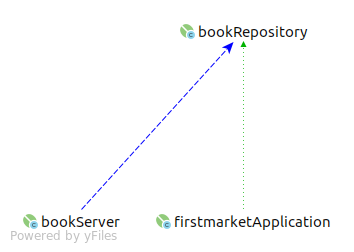
\includegraphics[width=0.6\textwidth]{di_bookRepository}
		\caption{Creación e inyección de dependencias en BookRepository}
		\label{fig:di_bookRepository}
	\end{figure}

	\begin{figure}[htb!]
		\centering
		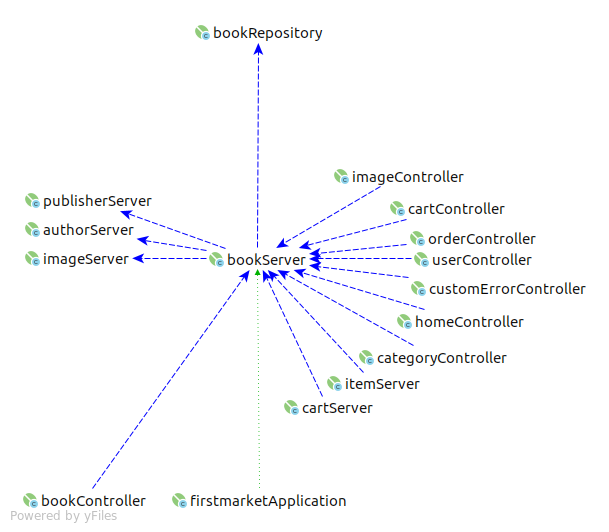
\includegraphics[width=\textwidth]{di_bookServer}
		\caption{Creación e inyección de dependencias en BookServer}
		\label{fig:di_bookServer}
	\end{figure}

	\begin{figure}[htb!]
		\centering
		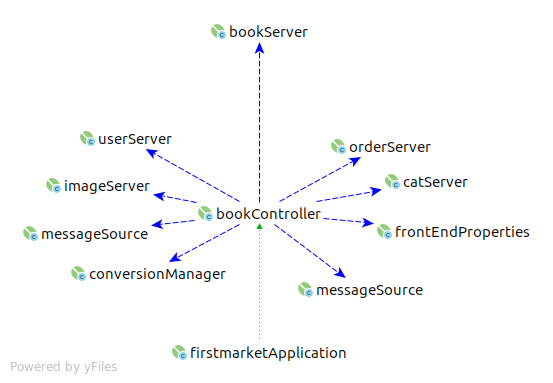
\includegraphics[width=\textwidth]{di_bookController}
		\caption{Creación e inyección de dependencias en BookContoller}
		\label{fig:di_bookController}
	\end{figure}
    
    \subsubsection{Capas funcionales} \label{sec:design_layer}
    Otro paso importante dado en la dirección de separar las responsabilidades es la división funcional del código en tres capas: web, negocio y persistencia. Estas capas están contenidas dentro del paquete \emph{core}, y están inspiradas en el patrón de diseño \emph{Fron Controller}, que es el que ordena, a su vez, la infraestructura web que proporciona Spring Framework (ver sección \ref{sec:springframework}).
    
    \begin{figure}[htb!]
    	\centering
    	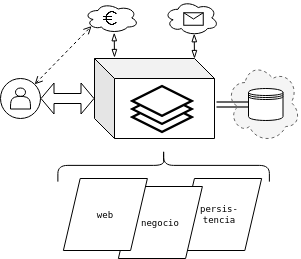
\includegraphics[width=0.75\textwidth,keepaspectratio]{desing_layer}
    	\caption{Modelo del sistema en capas funcionales}
    	\label{fig:desing_layer}
    \end{figure}
    
    La capa web se encarga de gestionar las peticiones HTTP encauzadas a través del \emph{DispatcherServler} y de resolver y generar el contenido HTML. A parte de toda la infraestructura que ofrece Spring Framework para esta tarea, se ha desarrollado una serie de \emph{controladores} (anotados con \emph{@Controller}), contenidos en el paquete \emph{core.controller} (ver figura \ref{fig:package_controller}), que sirven un conjunto de \emph{vistas}, contenidas en \emph{classpath: resources/templates}. Esta capa recibe el servicio de la capa de negocio.
    	
   	\begin{figure}[htb!]
   		\centering
   		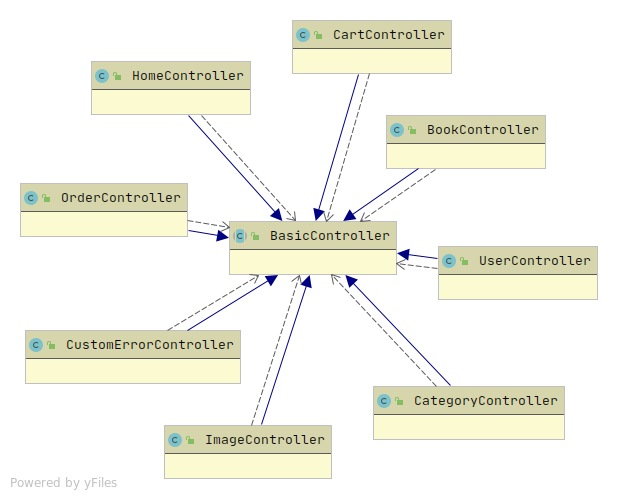
\includegraphics[width=0.7\textwidth,keepaspectratio]{package_controller}
   		\caption{Diagrama del paquete core.controller}
   		\label{fig:package_controller}
   	\end{figure}

   	\begin{figure}[htb!]
   		\centering
   		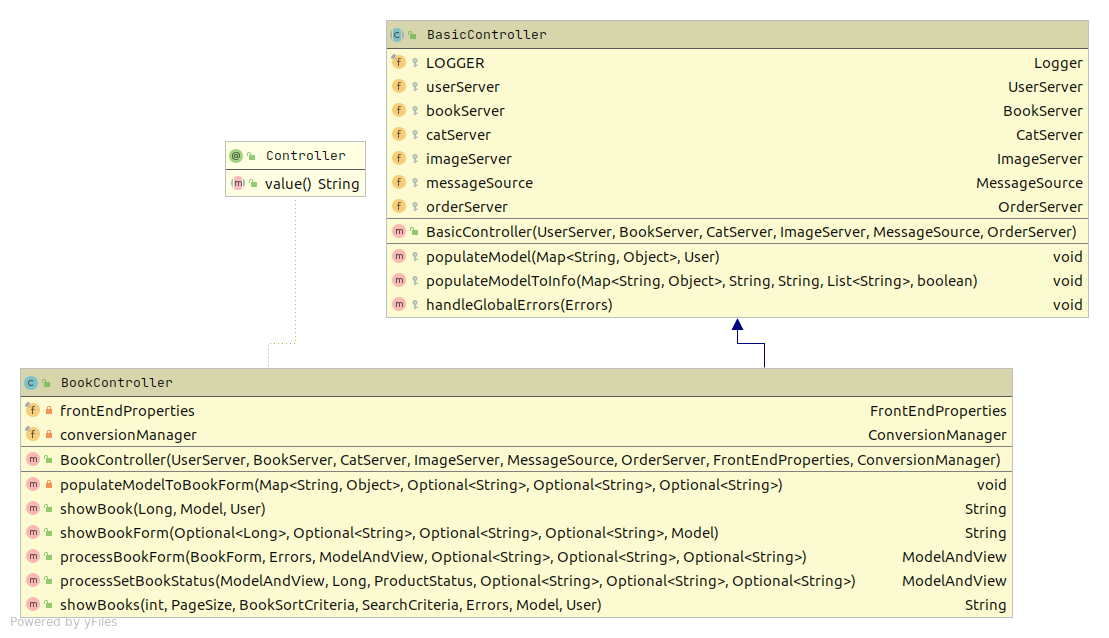
\includegraphics[width=\textwidth,keepaspectratio]{detail_bookController}
   		\caption{Detalle de la clase BookController}
   		\label{fig:detail_bookController}
   	\end{figure}
    	
   	En la capa de negocio reside la lógica (objetos anotados con \emph{@Service}) que modela el funcionamiento de una tienda de libros a través del código contenido en el paquete \emph{core.service} (ver figura \ref{fig:package_service}). Esta capa da servicio a la capa web y a sí misma, mientras que se apoya en el servicio que le ofrece la capa de persistencia.
    	
   	\begin{figure}[htb!]
		\centering
		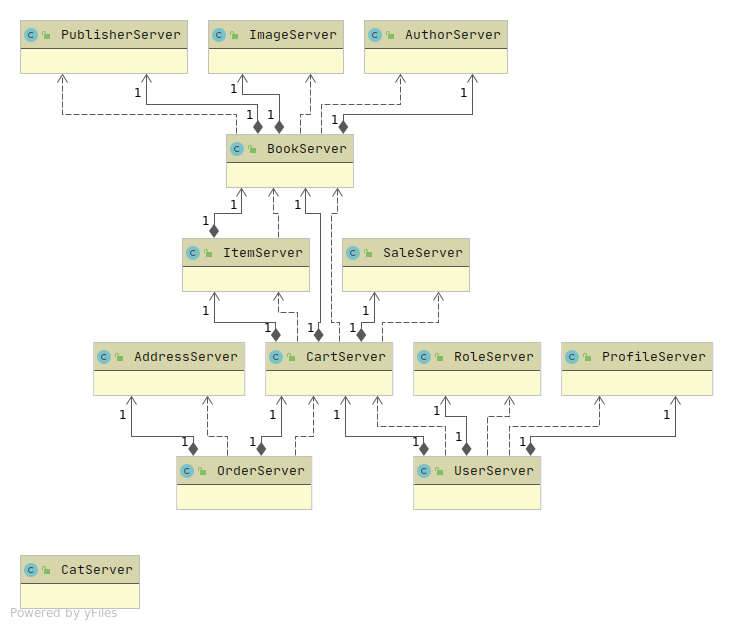
\includegraphics[width=\textwidth,keepaspectratio]{package_service}
		\caption{Diagrama del paquete core.service}
		\label{fig:package_service}
	\end{figure}

	\begin{figure}[htb!]
		\centering
		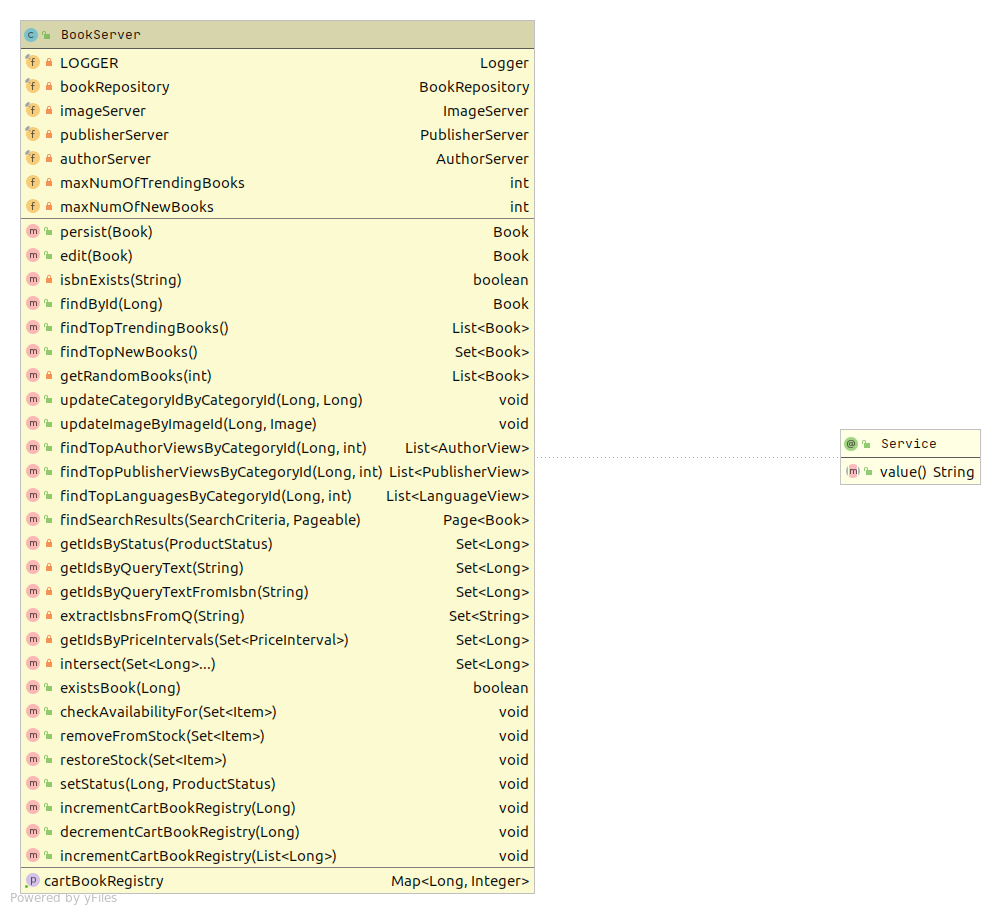
\includegraphics[width=\textwidth,keepaspectratio]{detail_bookServer}
		\caption{Detalle de la clase BookServer}
		\label{fig:detail_bookServer}
	\end{figure}

   	La capa de persistencia toma el control de todos los aspectos relacionados con la solución concreta de almacenamiento y manipulación de los datos (objetos anotados con \emph{@Repository}). Esta capa presta servicio a la capa de negocio mediante un conjunto de interfaces definidas en \emph{core.data} (ver figura \ref{fig:package_data}).
    	
   	\begin{figure}[htb!]
   		\centering
   		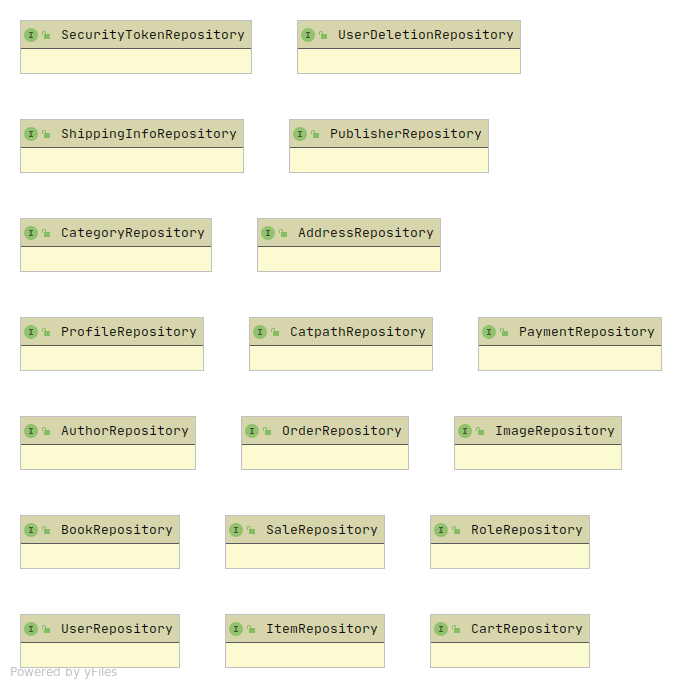
\includegraphics[width=\textwidth,keepaspectratio]{package_data}
   		\caption{Diagrama del paquete core.data}
   		\label{fig:package_data}
   	\end{figure}
   	
   	\begin{figure}[htb!]
   		\centering
   		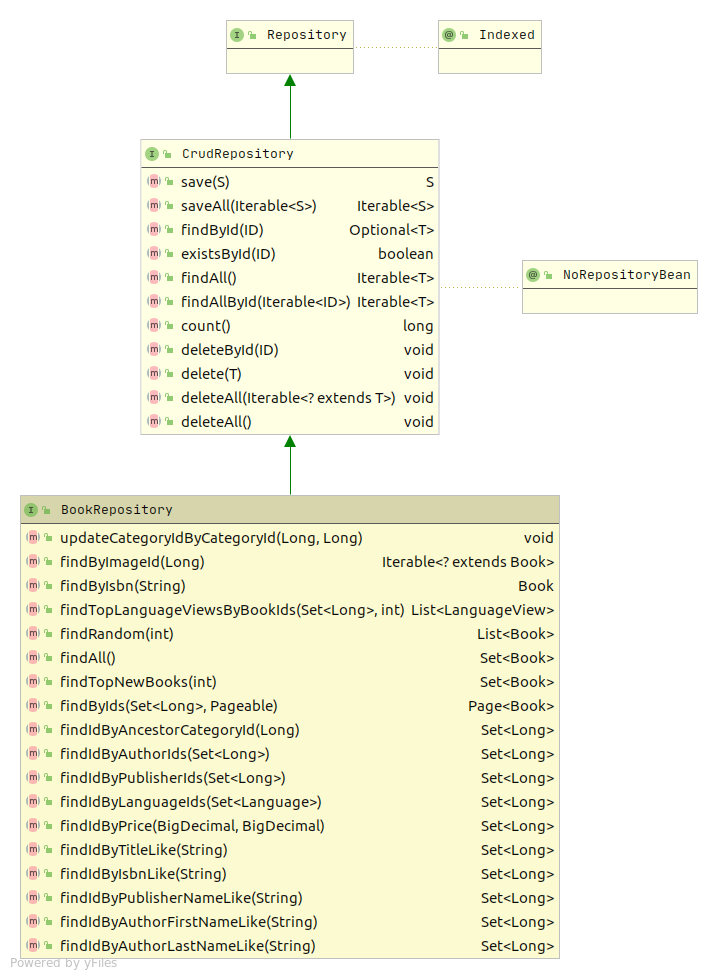
\includegraphics[width=\textwidth,keepaspectratio]{detail_bookRepository}
   		\caption{Detalle de la interfaz BookRepository}
   		\label{fig:detail_bookRepository}
   	\end{figure}
    	
    
    \subsection{Modelo de Datos}
    Para dar solución al problema presentado (la venta de libros online) se ha realizado un modelado de entidades del mundo real. Estas entidades se encuentran definidas en el paquete \emph{core.model}. En la figura \ref{fig:package_model} se muestra el diagrama de clases de este paquete. Este modelo encuentra una traducción directa en las entidades gestionadas en la base datos. En las figuras \ref{fig:er_simple_diagram} y \ref{fig:er_expanded_diagram} se ofrecen, respectivamente, los diagramas entidad relación sin y con las propiedades de los objetos visibles.
    
    \begin{figure}[htb!]
    	\centering
    	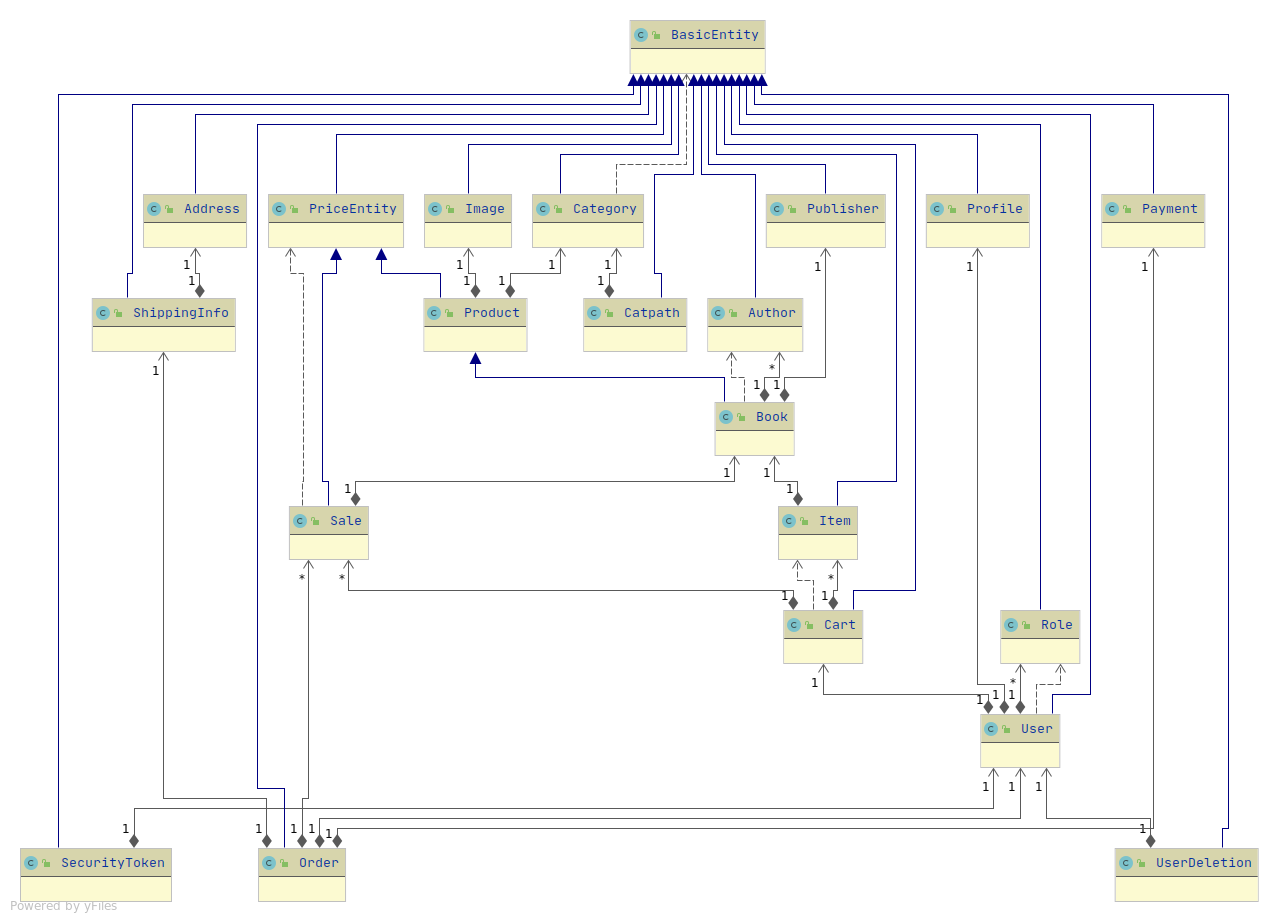
\includegraphics[height=\textwidth,angle=90,origin=c]{package_model}
    	\caption{Diagrama de clases del paquete core.model}
    	\label{fig:package_model}
    \end{figure}

	\begin{figure}[htb!]
		\centering
		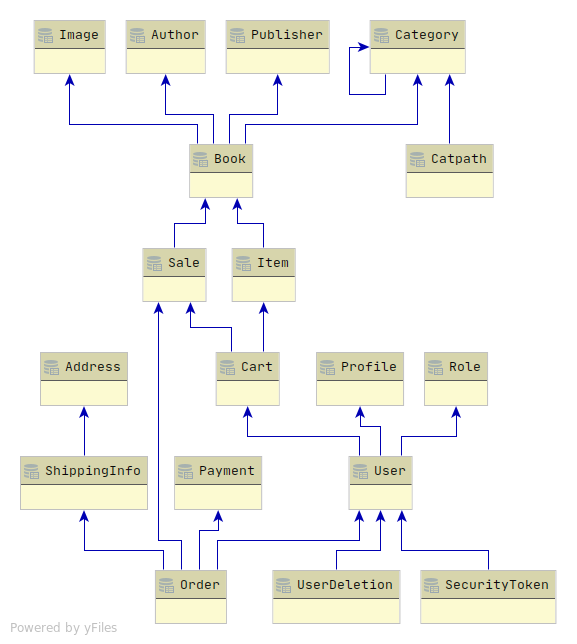
\includegraphics[width=\textwidth,keepaspectratio]{er_simple_diagram}
		\caption{Diagrama entidad-relación}
		\label{fig:er_simple_diagram}
	\end{figure}

	\begin{figure}[htb!]
		\centering
		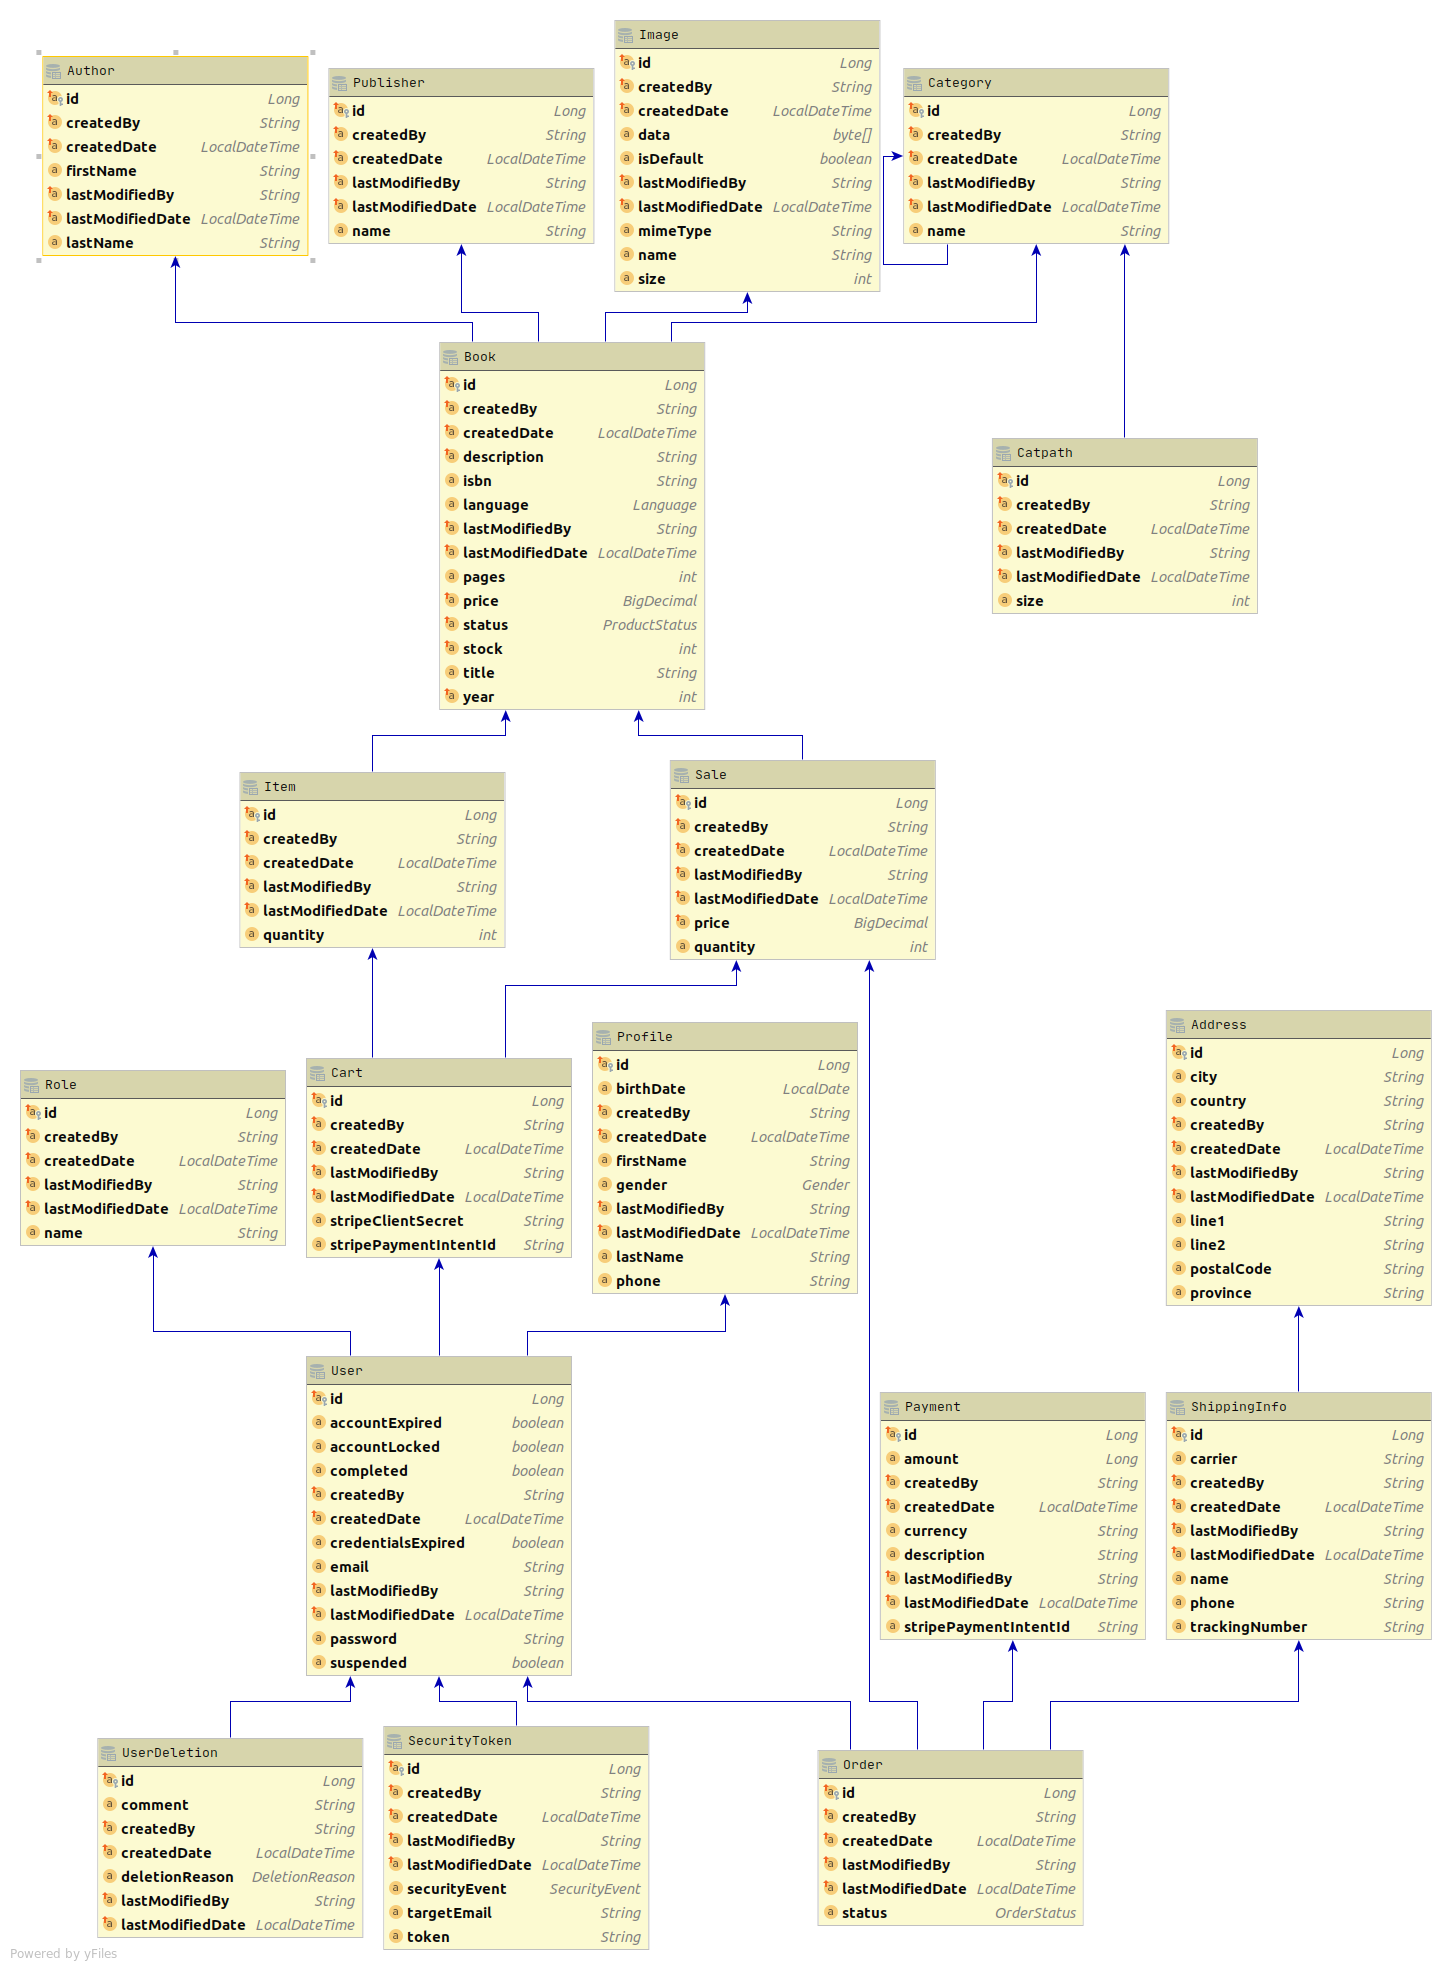
\includegraphics[width=\textwidth,keepaspectratio]{er_expanded_diagram}
		\caption{Diagrama entidad-relación expandido}
		\label{fig:er_expanded_diagram}
	\end{figure}

    % IMPLEMENTACION
    \section{Implementación}
    La materialización del análisis y diseño detallado en las secciones anteriores lo conforma el conjunto software que se incluye en el CD distribuido con la presente memoria. No obstante, en este apartado se ha querido comentar ciertos aspectos relevantes, que por la dificultad presentada y/o por el papel clave dentro de la aplicación merecen mención especial.
    
    \subsection{Control de Concurrencia}
    Uno de los aspectos más críticos para el correcto funcionamiento de una tienda online es el control del stock de productos y del proceso de realización de una compra. Muchos usuarios, quizás simultáneamente, pueden añadir productos a sus cestas y proceder a su compra. La aplicación debe garantizar que estas acciones se realicen de forma a conservar en todo momento la consistencia de los datos.
    
    \begin{figure}[hbt!]
    	\centering
    	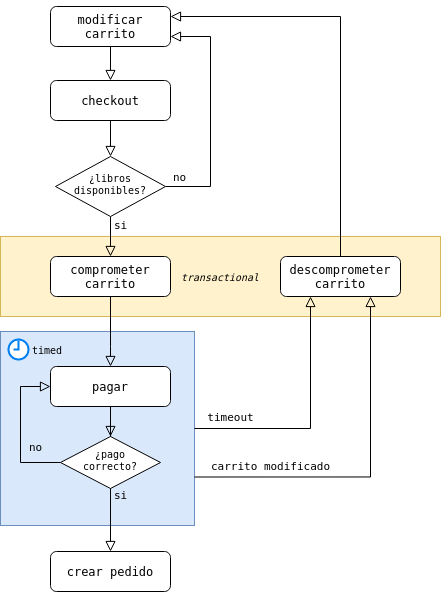
\includegraphics[width=0.7\textwidth,keepaspectratio]{cart_concurrent}
    	\caption{Diagrama del proceso de finalización de una compra}
    	\label{fig:cart_concurrent}
    \end{figure}
    
    Como se puede apreciar en la figura \ref{fig:cart_concurrent}, cuando un usuario decide proceder con el pedido de los libros contenidos en su cesta, lo primero que hace el sistema es comprobar que esos libros están disponibles. Pueden no estarlo por dos motivos, a saber, que estén agotados en ese momento o que el administrador de la aplicación web los haya deshabilitado (además, en este último caso el sistema automáticamente retira de la cesta dichos libros al detectar dicha situación). Si alguno de estos escenarios ocurriese la aplicación informaría al usuario en la propia vista de la cesta, sin avanzar a la vista de checkout, tal como se muestra en la figura \ref{fig:cart_alert}.
    
    \begin{figure}[hbt!]
    	\centering
    	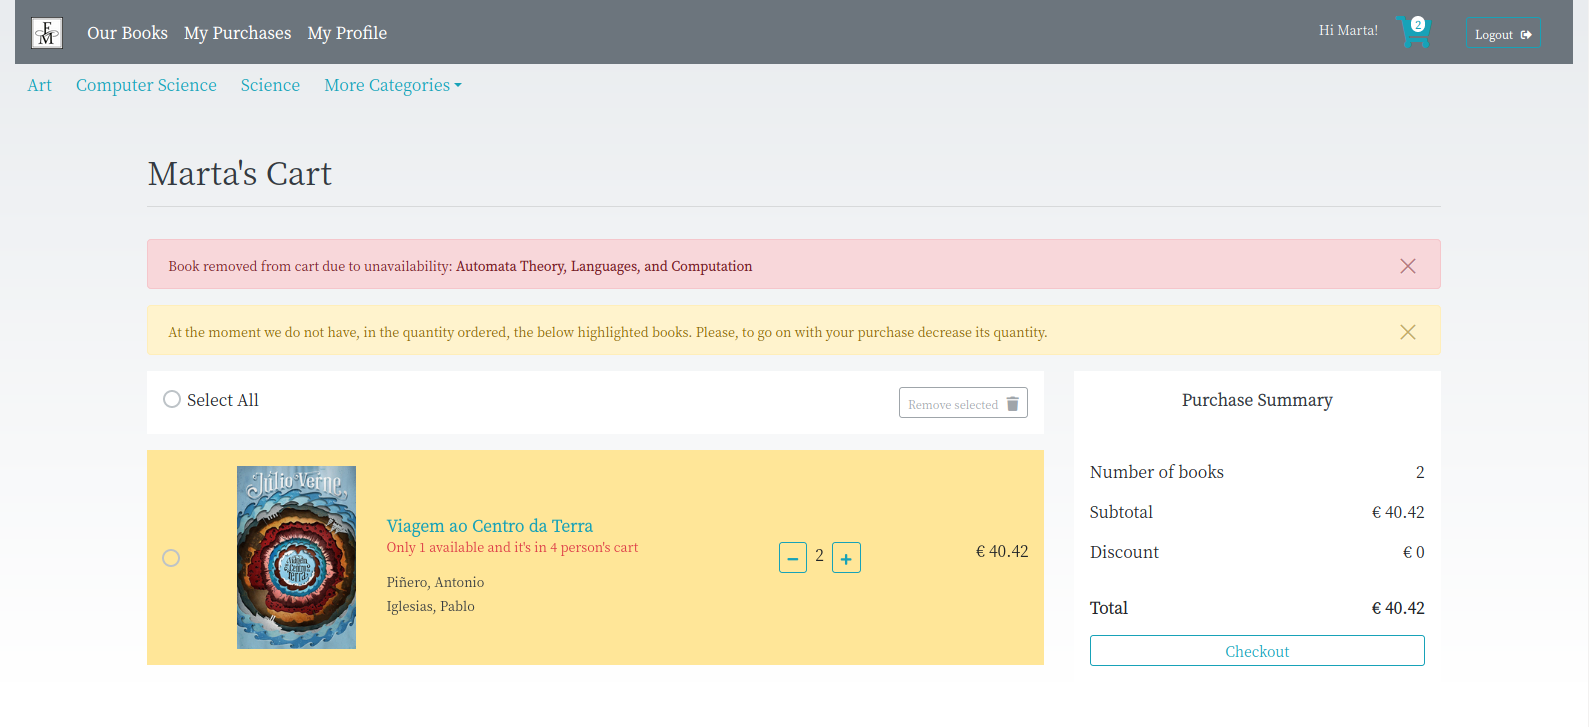
\includegraphics[width=\textwidth]{cart_alert}
    	\caption{Aviso por pantalla de no disponibilidad de libros}
    	\label{fig:cart_alert}
    \end{figure}
    
    Tras comprobar que los libros están disponibles el sistema \textbf{compromete} la cesta. Este es el paso fundamental donde se garantiza la consistencia. El sistema se compromete con el usuario a que si este finaliza la compra (dentro de un tiempo establecido) se le entregarán los libros seleccionados y al precio actual. Internamente, lo más destacado que el sistema realiza se recoge en:
    
    \begin{itemize}
    	\item[-] Se actualiza el stock, sustrayendo los libros en las cantidades correspondientes.
    	\item[-] Se crea en la base de datos una entidad \emph{sale} por cada item de la cesta, para así capturar el estado (principalmente el precio) de los libros en ese momento.
    	\item[-] Se contacta con Stripe para crear un nuevo \emph{Payment Intent}.
    	\item[-] Se activa el contador de tiempo disponible para finalizar la compra.
    \end{itemize}
    
    Todas estas acciones que realiza el sistema para comprometer la cesta las lleva a cabo de forma transaccional, apoyándose en la API de Spring Data JPA (ver \ref{sec:springdata}). Las transacciones software se describen en términos de las características ACID, del acrónimo en inglés de Atomicity, Consistency, Isolation, y Durability:
    
    \begin{itemize}
    	\item[-] Atomicity. Cada paso en la secuencia de acciones realizadas dentro de los límites de una transacción deben completarse con éxito o todo el trabajo debe
    	retroceder. La finalización parcial no es posible, o sucede todo o no sucede nada.
    	\item[-] Consistency. Los recursos de un sistema deben estar en un estado coherente, no corrupto, tanto en el inicio como en la finalización de una transacción.
    	\item[-] Isolation. El resultado de una transacción no debe ser visible para otras transacciones hasta que la primera se confirme con éxito.
    	\item[-] Durability. El resultado de una transacción comprometida debe hacerse permanente, independientemente a cualquier fallo del sistema.
    \end{itemize}
    
    Una vez comprometida la cesta, que otro usuario modifique el stock (ya sea un cliente al comprar un libro o el administrador al variar el stock), o que el administrador varíe el precio de algún libro de los recién comprometidos, o que incluso deshabilite alguno de estos libros, sería transparente para el usuario que acaba de comprometer su cesta. Mientras dure el tiempo disponible para finalizar la compra, la cesta comprometida es un contrato inmodificable. En este punto pueden suceder dos cosas: 
    
    \begin{enumerate}
    	\item El usuario completa el formulario de checkout y paga correctamente dentro del plazo, en cuyo caso se tramitaría el nuevo pedido.
    	\item El tiempo disponible para finalizar el pago se agota sin haber sido realizado, o el usuario, en la vista de la cesta, modifica las cantidades de los libros. Ante ambos eventos el sistema procede a \textbf{descomprometer} la cesta, abortándose de facto la compra.
    \end{enumerate}
    
    El procedimiento de descomprometer la cesta es el inverso al de comprometerla, y también se realiza transaccionalmente. Así, lo más destacado que el sistema lleva a cabo internamente en este proceso se resume en:
    
    \begin{itemize}
    	\item[-] Se actualiza el stock, aumentando los libros en las cantidades correspondientes.
    	\item[-] Se eliminan las entidades \emph{sale} correspondientes de la base de datos.
    	\item[-] Se contacta con Stripe para cancelar el \emph{Payment Intent}.
    \end{itemize}

    \subsection{Persistencia y Visualización de Datos Jerárquicos}
    Desde muy pronto se reparó en la necesidad de gestionar en la base de datos información con relaciones de jerarquía, ya que las categorías de los libros están organizadas de esta manera. Además, si se implementase la funcionalidad de que los usuarios pudiesen añadir comentarios a los libros, con capacidad de respuestas anidadas, también se estaría en el escenario de estructuras jerárquicas.
    
    Tal como se explica con detalle en [bib ref], existen diversas formas de dar solución a esta necesidad, cada una de ellas con sus puntos fuertes y sus debilidades. La idoneidad de una solución frente a otra viene en gran medida determinada por la cantidad de información jerárquica a gestionar y por la frecuencia o importancia relativa de las operaciones de lectura, creación, actualización y eliminación.
    
    Si los datos jerárquicos son siempre de pequeño tamaño y las operaciones son principalmente de lectura, una solución sería cargarlos en memoria principal y gestionarlos desde allí con alguna estructura de datos apropiada. Este podría argumentarse que es el caso de la información de las categorías de los libros, ya que en principio estas no superarían a lo sumo algunas decenas de centenas, y la actividad principal realizada sería la lectura. La frecuencia con que el administrador de la tienda crea, modifica o elimina una categoría es despreciable respecto de la frecuencia con que las categorías son leídas por los usuarios en general.
    
    Por otro lado, si se implementase la funcionalidad de los comentarios anidados, el escenario es claramente diferente. La cantidad de información es potencialmente mucho mayor, con lo que trabajar directamente en memoria principal no es una opción. Además, las operaciones de creación, modificación y eliminación cobran mayor protagonismo.
    
    La solución más común en este caso se conoce como listas de adyacencia, y no es otra cosa que añadir a cada entidad una referencia (clave extranjera) al id de su predecesor jerárquico. El problema de esta solución es que escala muy mal a medida que aumenta la profundidad del árbol. Imagínese que se tiene un hilo de comentarios arbitrariamente profundo, el cual precisaría de consultas recurrentes por cada nivel si se pretendiera extraer todo el hilo (algo habitual en estos sistemas de comentarios), ya que a priori se desconoce la profundidad. Sin embargo, existen métodos para extraer todo el hilo de comentarios con una sola consulta (en general, extraer cualquier subárbol), como se verá a continuación.
    
    La funcionalidad de que los libros estén clasificados por categorías es imprescindible para la aplicación, y en consecuencia ha sido implementada. No es el caso de los comentarios. No obstante, en un intento de hacer la aplicación fácilmente ampliable en este sentido, y dado que se trata de un proyecto académico, se optó por una solución que fuese eficiente y versátil: la denominada \textbf{Closure Table}.
    
    La idea principal es mantener la información de las relaciones entre las entidades en una tabla diferente. Es decir, por una parte se encuentra la tabla \emph{category} y por otra la tabla \emph{catpath}. En la primera se almacena la información relativa a las categorías (su id, nombre, etc), mientras que en la segunda se almacena la información de los caminos en el árbol de categorías. De todos los caminos, incluso de una categoría consigo misma. Así, por cada fila en la tabla \emph{catpath} se tiene el identificador del ancestro (clave extranjera de la tabla \emph{category}), el identificador del descendiente (también clave extranjera de la tabla \emph{category}) y el tamaño del camino. Para una relación de una categoría consigo misma el tamaño del camino es 0, para una relación directa el tamaño es 1, abuelo-nieto es 2 y así sucesivamente.
    
    \begin{figure}[htb!]
    	\centering
    	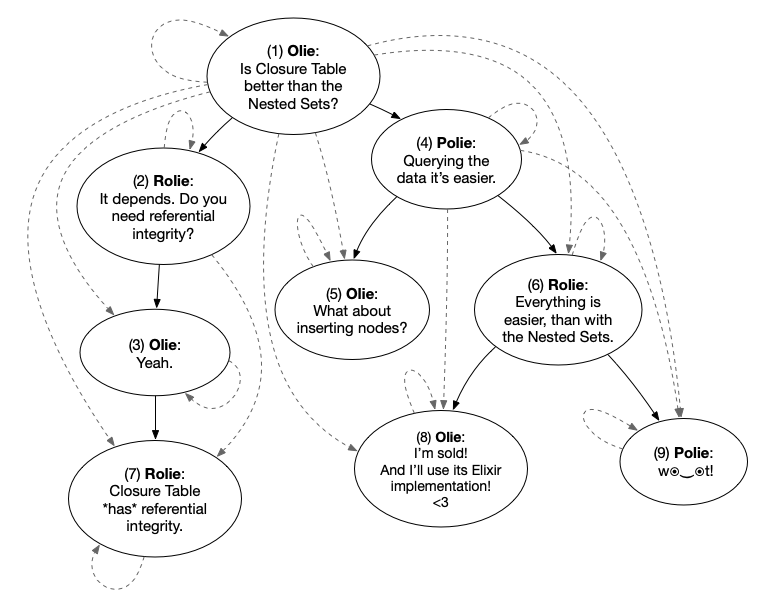
\includegraphics[width=0.7\textwidth]{closure_table}
    	\caption{Diagrama de conexiones registradas en una closure table}
    	\label{fig:closure_table}
    \end{figure}
    
    Esta solución es la más versátil y rápida de todas las mostradas en [bib ref], permitiendo incluso a un nodo pertenecer a varios árboles. Sin embargo, estos beneficios los consigue a costa de espacio. Este consumo puede ser importante si la estructura almacena jerarquías muy profundas.
    \\
    
    No obstante todo lo discutido con anterioridad, la solución real implementada para el trato específico de las categorías es triple (ver listado \ref{list:sql_cat}): Closure table, lista de adyacencia y trabajo en memoria principal con una estructura de datos en árbol. Esto es así por una cuestión de eficiencia y por desarrollar experiencia en el uso de estas soluciones.
    \\
    
    \begin{lstlisting}[caption=Tablas que gestionan las categorías,label=list:sql_cat]
    create table category (
    	id bigint not null, 
    	created_by varchar(255), 
    	created_date timestamp, 
    	last_modified_by varchar(255), 
    	last_modified_date timestamp, 
    	name varchar(255), 
    	parent_id bigint, 
    	primary key (id)
    );
    	
    create table catpath (
    	id bigint not null, 
    	created_by varchar(255), 
    	created_date timestamp, 
    	last_modified_by varchar(255), 
    	last_modified_date timestamp, 
    	size integer not null, 
    	ancestor_id bigint, 
    	descendant_id bigint, 
    	primary key (id)
    );
    
    alter table category 
    	add constraint fk_parentIdOnCategory foreign key (parent_id) references category(id)
    ;
    
    alter table catpath 
    	add constraint fk_ancestorIdOnCatpath foreign key (ancestor_id) references category(id)
    ;
    
    alter table catpath 
    	add constraint fk_descendantIdOnCatpath foreign key (descendant_id) references category(id)
    ;
    \end{lstlisting}
    
    Aparejado con el problema descrito en los párrafos anteriores se encuentra el de presentar al usuario dicha información jerárquica. Muy al principio del desarrollo de este proyecto se utilizó la tecnología de plantillas Java Server Pages para general el contenido HTML, la cual permite insertar en las vistas código Java de servidor. Así, se desarrolló una vista que contenía una función recursiva que permitía generar código HTML que mostrase la estructura anidada de las categorías. Pero esta aproximación de mezclar HTML y código Java de servidor es considerada una mala práctica y está en desuso.
    
    Posteriormente se adoptó el uso de Thymeleaf como motor de plantillas (ver \ref{sec:thymeleaf}), que no contempla esta posibilidad de insertar código de servidor en las vistas (al menos de la manera tan natural como lo permite JSP). Thymeleaf permite generar contenido \emph{lineal} (una lista, por ejemplo) haciendo uso de la directiva \emph{th:each}, que hace la veces de bucle \emph{for}, pero para generar contenido \emph{anidado} no dispone de ninguna funcionalidad nativa.
    
    Por todo lo anterior, para resolver este problema se optó por desarrollar código JavaScript (\emph{categoriesBuilder.js}) que se encargase, en el cliente, de construir y conectar, entre sí y al lugar apropiado en \emph{categories.html} (ver línea 15 del listado \ref{list:html_categories}), los componentes DOM necesarios para mostrar la estructura anidada de las categorías.
    \\
    
    \begin{lstlisting}[caption=Contenido principal de la vista categories.html,label=list:html_categories]
    <div class="container-fluid fm-content">
	    ...
	    <!-- main content -->
	    <div class="row">
		    <div class="col-sm-1"></div>
		    <div class="col-sm-10" id="root-hook">
			    <!-- new category -->
			    <div class="my-2 d-flex">
				    <a class="btn btn-outline-secondary align-center px-4 ml-auto" th:href="@{/admin/categoryForm}">
				    	<i class="fas fa-folder-plus fa-lg mr-4"></i>New Category
				    </a>
			    </div>
			    <hr/>
			    <!--
			    js dynamic generated content here
			    -->
		    </div>
		    <div class="col-sm-1"></div>
	    </div>
	    ...
    </div>
    \end{lstlisting}
    
    Como resultado, el administrador de la aplicación web puede visualizar la estructura jerárquica de las categorías a través de desplegables anidados, como se muestra en la figura \ref{fig:nested_categories}.
    
    \begin{figure}[htb!]
    	\centering
    	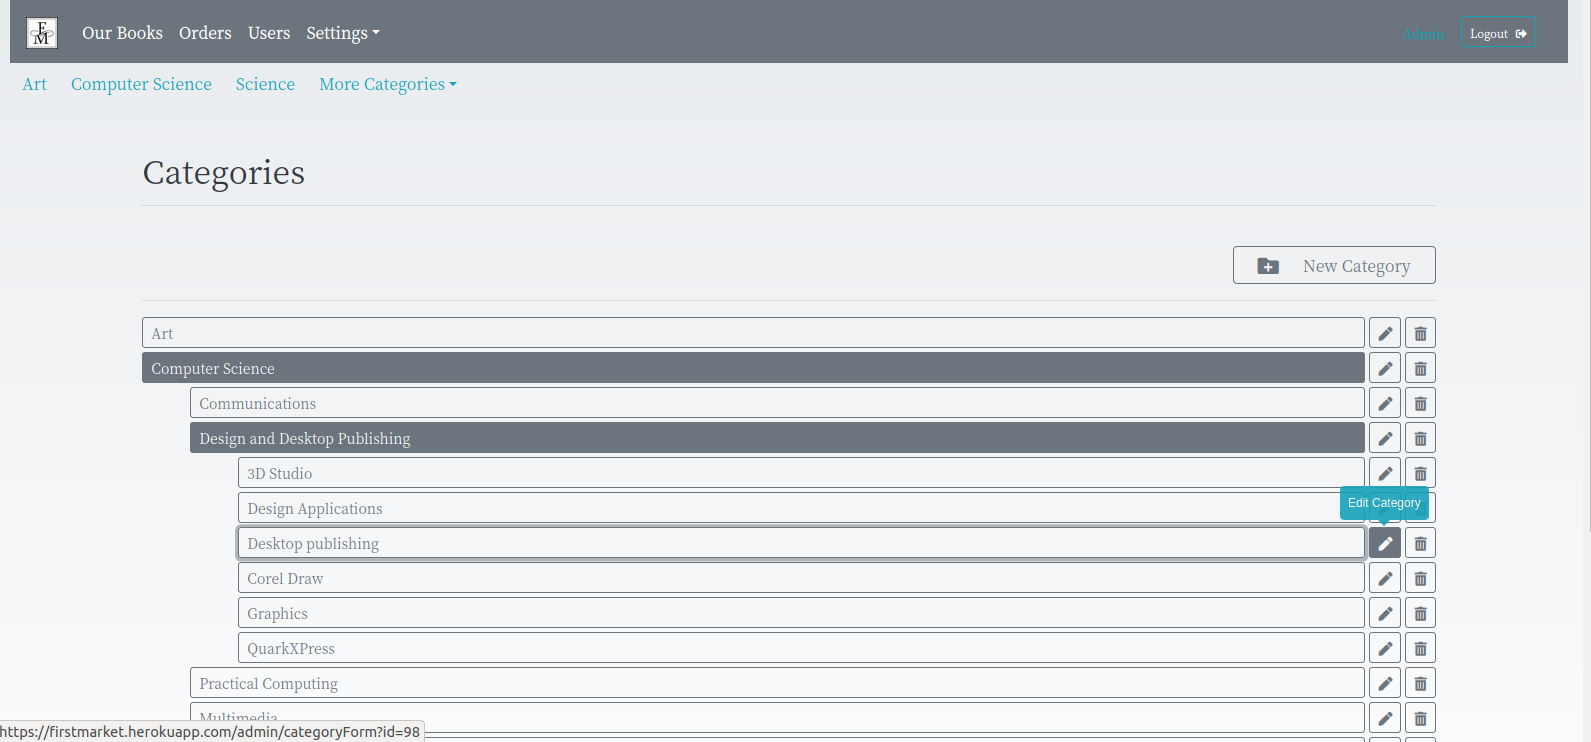
\includegraphics[width=\textwidth]{nested_categories}
    	\caption{Visualización de la estructura anidada de las categorías}
    	\label{fig:nested_categories}
    \end{figure}
    
    \subsection{Experiencia de Usuario Mejorada}
    Uno de los requisitos básicos de la aplicación web desarrollada es el de permitir a los usuarios gestionar su compra mediante el uso de una cesta virtual, que sirva de almacenamiento para la compra en curso. Esta funcionalidad permite a los usuarios:
    
    \begin{itemize}
    	\item[-] Añadir libros a la cesta. Esto se puede realizar desde cualquier vista que muestre información de un libro, a saber, la página de inicio, la página de resultados de búsqueda y la página de detalles de un libro.
    	\item[-] Modificar la cantidad de un libro en la cesta, o eliminar un libro de la cesta. Estas acciones se pueden realizar desde la vista de la cesta de un usuario.
    \end{itemize}
    
    Para la gestión de estas acciones, la arquitectura clásica de petición de un recurso por parte del cliente y respuesta con contenido HTML por parte del servidor (con su consecuente refresco de la página) se juzgó inapropiada. Un usuario que esté visualizando la página de su cesta y aumente en una unidad un libro tendría que esperar, para ver el resultado de dicho aumento, a que el servidor responda con el nuevo contenido HTML y que el navegador lo renderice, todo ello para únicamente cambiar unos pocos números respecto de la página previa. Situaciones similares ocurren en el caso de disminuir la cantidad de un libro, o eliminarlo de la cesta por completo. Peor aún es el caso del usuario que decide añadir un libro a su cesta, ya que el contenido HTML por el que debiera esperar sería igual (salvo el icono del número de elementos en la cesta) al de la página desde donde se solicita tal acción.
    
    En este contexto, y como pretexto perfecto para su estudio, se decidió desarrollar estas acciones con tecnología Ajax (ver \ref{sec:ajax}), de forma que no tenga lugar el refresco de la página en la que el usuario se encuentre. Así, el script \emph{ajaxCart.js} se encarga, entre otras cosas, de actualizar el DOM de la vista de la cesta del usuario, \emph{cart.html}, de manera consistente con las acciones que este realice, mientras que el script \emph{ajaxAddBook.js} gestiona el DOM de las citadas vistas desde las cuales es posible añadir libros a la cesta. Ambos scripts establecen en background la comunicación con el servidor, de forma transparente al usuario, haciendo uso del objeto \emph{XMLHttpRequest}, tal como muestra el extracto de \emph{ajaxCart.js} mostrado en el listado \ref{list:js_ajax}.
    \\
    
    \begin{lstlisting}[language=JavaScript,caption=Comunicación Ajax con el servidor,label=list:js_ajax]
    xmlHttpRequest = new XMLHttpRequest();
    xmlHttpRequest.open("GET", url, true);
    xmlHttpRequest.setRequestHeader('isAjaxCartRequested', '1');
    xmlHttpRequest.send();
    xmlHttpRequest.onreadystatechange = function() {
    	if (this.readyState === 4 && this.status === 200) {
    		onHttpOk(action, id, this.responseText);
    	}
    	if (this.readyState === 4 && this.status === 401) {
    		onHttpUnauthorized();
    	}
    };
    \end{lstlisting}
    
    \subsection{Registro de Libros Referenciados en Cestas}
    En este apartado se describe una funcionalidad añadida que, si bien no estaba presente en los requisitos de la aplicación, se ha mostrado muy útil y de relativa facilidad de implementación. La inspiración provino, como se aprecia en la figura \ref{fig:etsy}, del portal de comercio electrónico \href{https://www.etsy.com}{Etsy}, al querer imitar su capacidad de informar de la situación en la que, para un producto determinado, queden igual o menos unidades en stock de las que están siendo referenciadas en cestas de los usuarios. Esto es, que un libro esté en la cesta de \emph{x} usuarios diferentes, que de ese mismo libro queden en stock \emph{y} unidades, y que \emph{x} sea igual o mayor que \emph{y}.
    
    \begin{figure}[htb!]
    	\centering
    	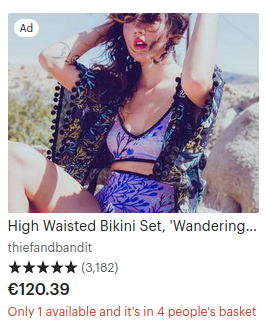
\includegraphics[width=0.5\textwidth]{etsy}
    	\caption{Aviso de producto escaso y demandado en Etsy.com}
    	\label{fig:etsy}
    \end{figure}
    
    Con este objetivo en mente, se pensó en tres alternativas para implementarlo. Por un lado, la solución trivial sería realizar una consulta a la base de datos para conocer de esta situación cada vez que se necesite mostrar al usuario información de un libro. En este sentido, sería necesario explorar las cestas de todos los usuarios, para cada libro del cual se requiera información. No es desacertado estimar que la frecuencia con se requiere información de libros en una tienda de libros sea alta. Además, el número de usuarios puede ser todo lo grande que se pueda. Por ello, esta solución sería bastante pobre en tiempo de respuesta.
    
    La segunda alternativa, con objeto a disminuir el tiempo de respuesta, sería aumentar la información de cada libro que se almacena en la base de datos, creando un nuevo campo en el que se contabilizase el número de referencias que a dicho libro le son realizadas en las cestas de los usuarios. Esta solución sería muy rápida, pero a costa de un uso redundante de los recursos de almacenamiento, puesto que la información necesaria \emph{ya} estaba en la base de datos.
    
    Finalmente, la tercera vía, que es la implementada, trata de aunar rapidez y no redundancia en la base de datos. Esto se consigue manteniendo la información necesaria en una estructura de datos llave-valor en memoria principal, sólo para los libros referenciados. La llave sería el \emph{id} de un libro, y el valor el número de referencias en cestas que posea. Los tiempos necesarios para consultar esta estructura de datos, así como para actualizarla, son muy bajos. Además, la base de datos se mantiene no redundante. Es cierto que existe un grado de redundancia, pero esta es ajena a la base de datos, y se limita a los libros que estén referenciados (en contraste con la segunda solución, en la que \emph{todos} los libros en la base de datos ampliaban su información).
    
    Esta estructura de datos es mantenida eficientemente por la clase \emph{BookServer}, como se aprecia en el listado \ref{list:java_cartbooks}, de manera que cada vez que algún usuario añade o elimina un libro de su cesta queda reflejado en el registro.
    \\
    
    \begin{lstlisting}[language=Java,caption=Gestión del registro de libros referenciados en cestas,label=list:java_cartbooks]
    @Service
    public class BookServer {
    
    	private final Map<Long,Integer> cartBookRegistry = new HashMap<>();
    	
    	...
    	
	    public void incrementCartBookRegistry(Long cartBookId) {
		    cartBookRegistry.merge(cartBookId, 1, (oldValue, defaultValue) -> ++oldValue);
	    }
	    
	    public void decrementCartBookRegistry(Long cartBookId) {
		    cartBookRegistry.computeIfPresent(cartBookId, (key, value) -> (value > 1L) ? --value : null);
	    }
	    
	    public void incrementCartBookRegistry(List<Long> cartBookIds) {
	    	cartBookIds.forEach(this::incrementCartBookRegistry);
	    }
	    
	    public Map<Long,Integer> getCartBookRegistry() {
	    	return cartBookRegistry;
	    }
    }
    \end{lstlisting}
    
    Así, este registro es utilizado para avisar a los usuarios cuando un libro presenta escasez y alta demanda, como se muestra en la figura \ref{fig:fm_cartBookRegistry_alert}. Pero también es usado como \textbf{medida de la popularidad} de los libros, empleándose este uso en la página de inicio de la aplicación. Es cierto que el parámetro \emph{popularidad} se puede definir de muchas maneras, y que sería conveniente que en él se reflejase el volumen de ventas en una ventana temporal local, pero como una primera aproximación de bajo coste al concepto funciona perfectamente.
    
    \begin{figure}[htb!]
    	\centering
    	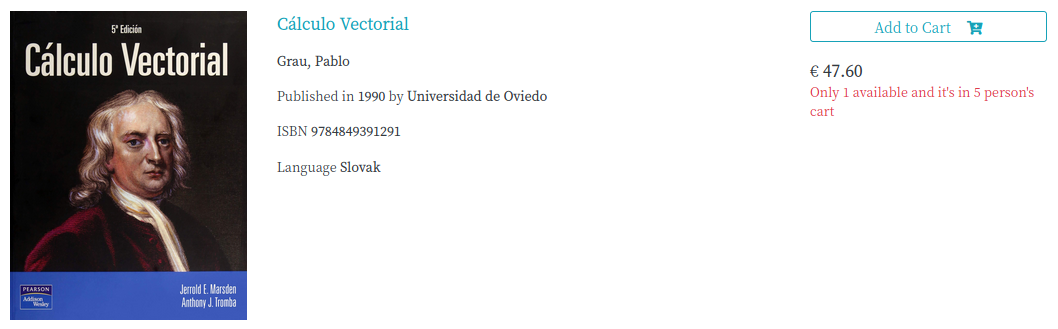
\includegraphics[width=\textwidth]{fm_cartBookRegistry_alert}
    	\caption{Aviso de producto escaso y demandado en FirstMarket}
    	\label{fig:fm_cartBookRegistry_alert}
    \end{figure}
    
    \subsection{Validación}
    Por validación se entiende las comprobaciones que la aplicación web hace sobre los datos que le son proporcionados externamente. El caso más común es cuando un usuario envía un formulario cumplimentado a la aplicación web, y esta, antes de procesar la información, comprueba que se cumplen ciertas reglas. Por ejemplo, puede requerirse que el campo de email sea efectivamente una dirección de correo válida, o que la fecha de nacimiento sea una fecha pasada válida (nadie puede nacer el 30 de febrero, por ejemplo). Esto se hace para garantizar la consistencia de los datos en la base de datos y por motivos de seguridad, como evitar ataques de inyección SQL.
    
    Esta comprobación se puede hacer tanto en cliente como en servidor. Desde el punto de vista de la seguridad, realizar la comprobación en servidor es obligatorio, ya que las comprobaciones en cliente son muy fácilmente circunvaladas. Por otro lado, desde el punto de vista de la experiencia de usuario es muy recomendable implementarla también en cliente, ya que permite al usuario tener un feedback mucho más rápido que si debiese esperar a que el servidor responda. En definitiva, la mejor práctica es implementar la validación tanto en backend como en frontend. Y así se ha hecho.
    \\
    
    Mucha es la información que FirstMarket tiene que validar, pero a grandes rasgos se puede dividir en numérica y textual. El primer grupo presenta poca dificultad, se trata de comprobar rangos de valores principalmente. Para el segundo grupo las expresiones regulares son el arma perfecta. En el archivo de configuración \emph{application.yml} se detallan las expresiones regulares y los rangos numéricos utilizados. A modo de ejemplo, la propiedad definida en este archivo de configuración que especifica la expresión regular contra la que validar las contraseñas se muestra en el listado \ref{list:regex_pw}.
    \\
     
    \begin{lstlisting}[caption=Expresión regular para las contraseñas,label=list:regex_pw]
    fm:
      validation:
        regex:
          password: ^(?=.*\d)(?=.*[a-z])(?=.*[A-Z]).{8,16}$
    \end{lstlisting}
    
    Así, esta expresión regular es utilizada por la aplicación web para comprobar, tanto en frontend como en backend, que cuando un usuario proporciona una nueva contraseña esta tenga una longitud de entre 8 y 16 caractéres e incluya al menos una minúscula, una mayúscula y un dígito.
    \\
    
    Existe un campo que destaca por su manera de ser validado. Se trata del ISBN (International Standard Book Number) de los libros. Este campo necesita validación en dos vertientes, a saber, sintáctica y semántica. La validación sintáctica se realiza utilizando las ya mencionadas expresiones regulares, pero para validar si se trata de un ISBN válido aún hay que calcular mediante un algoritmo concreto un dígito de control y ver si coincide con el último dígito del código. Los ISBN tuvieron 10 dígitos hasta diciembre de 2006, pero desde entonces tienen siempre 13 dígitos (ambas versiones con diferentes algoritmos de cálculo del dígito de control). Así pues, la validación debe dar soporte a ambos formatos de ISBN. A modo de ejemplo, en el listado \ref{list:js_isbn} se detalla la función JavaScript desarrollada para comprobar en el cliente el dígito de control.
    \\
    
    \begin{lstlisting}[language=JavaScript,caption=Validación del dígito de control del ISBN en cliente,label=list:js_isbn]
    const isbnChecksum = function() {
    	let chars, last, sum, check, i;
    	const isbn = document.getElementById("isbn");
    	if (isbn.checkValidity()) {
    		// Remove non ISBN digits, then split into an array
    		chars = isbn.value.replace(/[- ]|^ISBN(?:-1[03])?:?/g, "").split("");
    		// Remove the final ISBN digit from `chars`, and assign it to `last`
    		last = chars.pop();
    		sum = 0;
    		if (chars.length == 9) {
    			// Compute the ISBN-10 check digit
    			chars.reverse();
    			for (i = 0; i < chars.length; i++) {
    				sum += (i + 2) * parseInt(chars[i], 10);
    			}
    			check = 11 - (sum % 11);
    			if (check == 10) {
    				check = "X";
    			} else if (check == 11) {
    				check = "0";
    			}
    		} else {
    			// Compute the ISBN-13 check digit
    			for (i = 0; i < chars.length; i++) {
    				sum += (i % 2 * 2 + 1) * parseInt(chars[i], 10);
    			}
    			check = 10 - (sum % 10);
    			if (check == 10) {
    				check = "0";
    			}
    		}
    		if (check != last) {
    			alert("Error: Invalid ISBN checksum digit (" + last + "). Try with (" + check + ")");
    			isbn.focus();
    			isbn.value = isbn.value.substring(0, isbn.value.length - 1);
    		}
    	}
    };
    \end{lstlisting}
    
    
    % TECNOLOGIAS
    \section{Stack Tecnológico}
    En este apartado se ofrece un comentario del stack tecnológico con el que se ha llevado a cabo la aplicación web.

    \subsection{Spring} \label{sec:spring}
    Sin duda, Spring ha sido una de las tecnologías que más impacto ha tenido en el presente proyecto. En esta sección se pretende dar una idea lo más general y amplia posible de sus características.
    
    Lo primero a aclarar es qué se entiende por \emph{Spring}, ya que su significado puede variar dependiendo del contexto. Puede que se refiera en concreto al proyecto \emph{Spring Framework}, donde empezó todo allá por el año 2003, o al ecosistema completo formado por todos los \href{https://spring.io/projects}{proyectos} Spring, esto es, por Spring Framework más todos los otros proyectos Spring que se desarrollaron posteriormente utilizando como núcleo al primero.
    
    Los proyectos Spring usados en el desarrollo de la aplicación web han sido \emph{Spring Framework}, \emph{Spring Boot}, \emph{Spring MVC}, \emph{Spring Data} y \emph{Spring Security}.
    
    \subsubsection{Spring Framework} \label{sec:springframework}
    En este apartado se esbozará las principales características de esta parte fundamental dentro del ecosistema Spring, tomando para ello como principal fuente su propia \href{https://docs.spring.io/spring/docs/current/spring-framework-reference/}{documentación}.
    
    Tal como establecen sus autores, los principios de diseño que han guiado su desarrollo a lo largo del tiempo han sido:
    
    \begin{itemize}
    	\item[-] Estar orientado a permitir que se tomen las decisiones de diseño lo más tarde posible. Por ejemplo, permite cambiar la tecnología de persistencia sin alterar el código de la aplicación (esto fue constatado en el desarrollo de la aplicación web, al pasar de forma transparente, en una etapa bastante avanzada del proyecto, de MariaDB a PostgreSQL).
    	\item[-] Ser capaz de acomodar diferentes perspectivas de desarrollo. Spring es extensamente configurable, no imponiendo ningún estilo o manera de resolver los problemas.
    	\item[-] Ser altamente retrocompatible.
    	\item[-] Tomar muchas precauciones a la hora de diseñar las APIs, de forma que sean intuitivas y perduren a través de las diferentes versiones.
    	\item[-] Seguir los más altos estándares de calidad del código.
    \end{itemize}
    
    De todas las funcionalidades integradas dentro del proyecto Spring Framework, la más importante es el contenedor de Inversión de Control (inversion of control, IoC). Este concepto, tratado en la sección \ref{sec:ioc}, hace referencia a la capacidad de gestionar el ciclo de vida de los \emph{beans}, que es como en el ecosistema Spring se conoce a los objetos gestionados por el contenedor.
    
    La interfaz \emph{org.springframework.context.ApplicationContext}, que representa el contenedor de IoC de Spring, es la responsable de instanciar, configurar y ensamblar los \emph{beans}.
    
    Por su parte, el contenedor conoce qué objetos instanciar y cómo configurarlos y ensamblarlos entre sí a través de la lectura de metadatos de configuración especificados por el desarrollador.
    
    La figura \ref{fig:container_magic}, tomada de la documentación oficial, muestra un diagrama de alto nivel de cómo funciona lo explicado. Esto es, el código desarrollado en forma de POJOs (Plain Old Java Object) es gestionado en el contenedor de IoC según se haya especificado en los metadatos de configuración, produciendo como resultado una aplicación completamente funcional.
    
    \begin{figure}[hbt!]
    	\centering
    	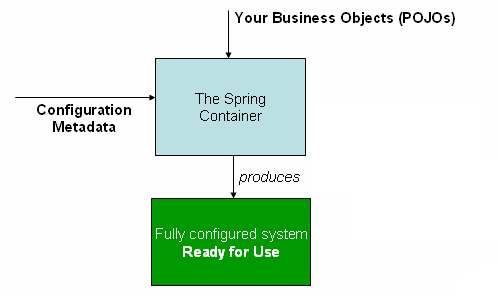
\includegraphics[width=0.8\textwidth,keepaspectratio]{container_magic}
    	\caption{Flujo de información en el contenedor de IoC}
    	\label{fig:container_magic}
    \end{figure}
    
    Existen diversas formas de especificar los metadatos de configuración. La manera original fue a través de un fichero XML, pero en la actualidad también se puede realizar con anotaciones insertadas en el código de la aplicación (añadido en la versión 2.5), o con código Java dedicado de configuración (añadido en la versión 3.0). El contenedor de IoC está completamente desacoplado de estos mecanismos de especificación de los metadatos de configuración.
    
    Existe la cuestión de qué tipo de configuración es mejor. La respuesta no es clara, ya que cada opción posee su dosis de ventajas e inconvenientes. Las anotaciones son la manera más concisa y quizás mas simple para un principiante, pero mezclan código de negocio con configuración del framework, algo que mina el principio de separación de responsabilidades. Además poseen el inconveniente de descentralizar la configuración, impactando negativamente en su mantenibilidad. La configuración con código Java permite un control centralizado, pero se pierde en facilidad y brevedad. Por su parte, los ficheros XML son inmejorables a la hora separar responsabilidades, pudiéndose alterar la configuración sin tocar una línea de código y, por tanto, sin tener que recompilar. El inconveniente de este sistema es el elevado tamaño y complejidad que muchas veces estos ficheros alcanzan, siendo además su curva de aprendizaje más pronunciada.
    
    En el desarrollo de la presente aplicación web se ha utilizado la configuración a través de anotaciones y de código Java dedicado. Además, se ha utilizado Spring Boot, lo que, como se verá, implica que una gran parte (la mayoría) de la configuración necesaria ha sido establecida por defecto.
    \\
    
    Además del contenedor de IoC, la aplicación web desarrollada hace uso de otras capacidades ofrecidas por Spring Framework:
    
    \begin{itemize}
    	\item[-] Publicación y escucha de eventos.
    	\item[-] Gestión de transacciones.
    	\item[-] Planificación de tareas.
    	\item[-] Validación.
    	\item[-] El framework de desarrollo web \emph{Spring Web MVC} (comúnmente conocido como simplemente Spring MVC).
    \end{itemize}

	Spring MVC, como muchos otros frameworks de desarrollo web, está implementado alineado con el patrón de diseño \emph{Front Controller}, donde un Servlet central, el llamado \emph{DispatcherServlet}, recibe las peticiones HTTP y delega su procesamiento a los componentes apropiados, en el caso de la presente aplicación los objetos anotados con \emph{@Controller}. Cada uno de estos objetos es responsable de llevar a cabo las acciones necesarias para cada \emph{endpoint} expuesto, apoyándose para ello en la capa de negocio, es decir, en los objetos anotados con \emph{@Service}. Como ya se explicó en la sección \ref{sec:design_layer}, estos objetos \emph{@Service} se apoyan, a su vez, en otros objetos de su clase y en objetos anotados con \emph{@Repository}, que actúan como puerta de entrada a los datos. Cumplida la lógica de negocio, el objeto \emph{@Controller} implicado devuelve el nombre de la vista a proporcionar como respuesta, así como los datos con los que poblarla. El motor de plantillas genera en este punto el contenido HTML, que es devuelto por el \emph{DispatcherServlet} al usuario.
	
	En resumen, Spring MVC ofrece la infraestructura \emph{Front Controller}, esto es, los objetos necesarios para resolver el mapeo de las peticiones HTTP a los métodos apropiados de los objetos \emph{@Controller}, los objetos encargados de resolver las vistas, los encargados del enlace de datos, etc, permitiendo al desarrollador centrarse en especificar la lógica de negocio.
    
    
    \subsubsection{Spring Boot}
    Este proyecto ha sido el gran avance de los últimos años dentro del universo Spring. De hecho, ha cambiado por completo el paradigma, permitiendo el desarrollo de aplicaciones totalmente funcionales en un espacio de tiempo dramáticamente inferior al necesario con anterioridad a su aparición. Tal como viene recogido en la \href{https://docs.spring.io/spring-boot/docs/current-SNAPSHOT/reference/html/}{documentación} oficial, sus principales objetivos son:
    
    \begin{itemize}
    	\item[-] Ofrecer una vía de entrada al uso de las tecnologías Spring radicalmente más rápida y sencilla.
    	\item[-] Proporcionar una configuración por defecto sensata, y al mismo tiempo de ágil modificación si los requisitos así lo necesitan.
    	\item[-] Ofrecer todo un abanico de funcionalidades transversales a la mayoría de aplicaciones, como los servidores embebidos.
    	\item[-] Supresión de la necesidad de configuración a través de ficheros XML.
    \end{itemize}

	Así, Spring Boot no es una alternativa a otros proyectos Spring. Su objetivo no es proporcionar nuevas soluciones para problemas ya resueltos, sino ofrecer una manera de mejorar el aprovechamiento del ecosistema entero, fomentando una experiencia de desarrollo que simplifique el uso de los módulos ya disponibles. Esto hace que Spring Boot sea una opción ideal para toda clase de desarrolladores, tanto los que ya están familiarizados con el ecosistema Spring como aquellos recién llegados, al permitirles adoptar las tecnologías de Spring de una manera simplificada. En este sentido, Spring Boot ha supuesto un vector de expansión de las tecnologías Spring, disminuyendo su barrera de entrada y maximizando el aprovechamiento de sus variadas funcionalidades.
    
    En gran medida, lo expuesto se consigue gracias a que Spring Boot ejercita el paradigma de diseño conocido como Convención sobre Configuración (\emph{Convention over Configuration, CoC}), o también como Código por Convención (\emph{Coding by Convention}). Este principio de diseño trata de disminuir el número de decisiones que el desarrollador debe tomar y aliviar así la complejidad de tener que configurar todas y cada una de las áreas que conforman una aplicación, todo ello sin necesariamente merma alguna en la flexibilidad. Así, el desarrollador sólo está llamado a especificar los aspectos no convencionales de la configuración de la aplicación, obteniendo como resultado inmediato un aumento en la productividad considerable.
    
    Conviene destacar también que Spring Boot permite ejecutar aplicaciones web sin necesidad de hacerlo en un contenedor de servlets externo o un servidor de aplicaciones, ya que el propio Spring Boot incluye un Tomcat embebido, el cual se despliega automáticamente en tiempo de ejecución.
    
    \subsubsection{Spring Data} \label{sec:springdata}
    \subsubsection{Spring Security}
    \subsection{Thymeleaf - HTML5} \label{sec:thymeleaf}
    \subsection{Bootstrap 4 - CSS3}
    \subsection{Stripe} \label{sec:stripe}
    \subsection{PostgreSQL}
    \subsection{JavaScript}
    \subsubsection{Ajax} \label{sec:ajax}
    \subsection{FontAwesome - Pretty Checkbox - Google Fonts}
    \subsection{Tecnologias Transversales}
    \subsubsection{Git}
    \subsubsection{Java 11}
    \subsubsection{Maven}
    Las librerías son ficheros que proporcionan una serie de funciones que simplifican el trabajo del programador y que suelen ser un elemento fundamental de cualquier desarrollo software. Normalmente, el desarrollador necesita saber qué librería usar y qué versión en particular. Además, una librería puede depender de otras para operar adecuadamente, lo que obliga a tener que gestionarlas para que no entren en conflicto entre sí.
    
    Para lidiar con este problema, existe una herramienta llamada Maven que se ocupa de la gestión de las distintas librerías mediante el uso de los llamados Artefactos o Artifacts, que son elementos que engloban las clases de una librería y la información necesaria para su óptima gestión (grupo, nombre, versión, otras dependencias...). Los Artifact se definen en el archivo POM.xml, que es el fichero que almacena toda la información del proyecto.
    
    Maven, por tanto, se encarga de descargar mediante un sencillo artefacto todas las librerías declaradas en el fichero POM.xml. Además, también hace posible la descarga de documentación relativa a estas librerías u otras dependencias subyacentes que no hayan sido definidas intencionadamente por el desarrollador.
    
    En última instancia, Maven usa las librerías descargadas para la compilación del proyecto.
    \subsubsection{IntelliJ IDEA}
    \subsubsection{Logback}
    \subsubsection{Lombok}
    \subsubsection{Guava}

    % DESPLIEGUE Y SEGURIDAD
    \section{Despliegue y Seguridad}
    En esta sección se aborda todos los aspectos relevantes en relación con el despliegue de la aplicación web, así como de las medidas de seguridad adoptadas.
        \subsection{Heroku Platform}
        La aplicación ha sido desplegada en Heroku.
            \subsubsection{Heroku-postgresql}
            \subsubsection{LogDNA}
            \subsubsection{Probely}
        \subsection{Spring Security}
        \subsection{HTTPS}
        \subsection{Cross-Site Request Forgery}
        \subsection{Brute-Force Authentication}

    % MANUALES
    \section{Manuales}
    En esta seccion se va a describir las cuestiones necesarias para facilitar el uso de la aplicacion web por parte de los usuarios
        \subsection{Usuario Cliente}
    aqui va la descripcion para el usuario cliente
        \subsection{Usuario Administrador}
    aquie se describe el uso del admin

	% PRESUPUESTO
	\section{Presupuesto}

    % MEJORAS Y AMPLIACIONES
    \section{Mejoras y Ampliaciones}
    Testar el software
    Sistema de valoracion por parte de los usuarios de los libros


\end{document}
